%%%%%%%%%%%%%%%%%%%%%%%%%%%%%%%%%%%%%%%%%%%%%%%%%%%%%%%%%%%%%%%%%%%%%%%%%%%%%
%%%%%%                                                                  %%%%% 
%%%%%%          Maqueta de memòria TFC/PFC de l'EETAC                   %%%%% 
%%%%%%                                                                  %%%%% 
%%%%%%%%%%%%%%%%%%%%%%%%%%%%%%%%%%%%%%%%%%%%%%%%%%%%%%%%%%%%%%%%%%%%%%%%%%%%%
%%%%%%%%%%%%%%%%%%%%%%%%%%%%%%%%%%%%%%%%%%%%%%%%%%%%%%%%%%%%%%%%%%%%%%%%%%%%%
%%                                                                         %%
%%          Autor: Xavier Prats i Menéndez (xavier.prats@upc.edu)          %% 
%%                  Technical University of Catalonia (UPC)                %%
%%                                                                         %%
%%%%%%%%%%%%%%%%%%%%%%%%%%%%%%%%%%%%%%%%%%%%%%%%%%%%%%%%%%%%%%%%%%%%%%%%%%%%%
%%      This work is licensed under the Creative Commons  Attribution-     %%
%%   -Noncommercial-Share Alike 3.0 Spain License. To view a copy of this  %% 
%%    license, visit http://creativecommons.org/licenses/by-nc-sa/3.0/es/  %%
%%    or send a letter to Creative Commons, 171 Second Street, Suite 300,  %%
%%                  San Francisco,California, 94105, USA.                  %%
%%%%%%%%%%%%%%%%%%%%%%%%%%%%%%%%%%%%%%%%%%%%%%%%%%%%%%%%%%%%%%%%%%%%%%%%%%%%%
%% Versió 2.1 - Juliol 2012                                                %%
%%%%%%%%%%%%%%%%%%%%%%%%%%%%%%%%%%%%%%%%%%%%%%%%%%%%%%%%%%%%%%%%%%%%%%%%%%%%%

%%% NOTA: els seguents packages son necessaris per utilitzar la
%%%       plantilla seguent:
%%%       ifthen,calc,helvet,pslatex,fancyhdr,nextpage,subfigure,tocloft,graphicx,url

%%% NOTA: Es possible que algunes distribuicions Linux o Windows.
%%%       no portin aquests paquets instal·lats per defecte.
%%%       En aquest cas els haureu d'instal·lar manualment.


%%%%%%%%%%%%%%%%%%%%%%%%%%%%%%%%%%%%%%%%%%%%%%%%%%%%%%%%%%%%%%%%%%%%%%%%%%%%%
% 1- INICIALITZACIÓ
%%%%%%%%%%%%%%%%%%%%%%%%%%%%%%%%%%%%%%%%%%%%%%%%%%%%%%%%%%%%%%%%%%%%%%%%%%%%%

\documentclass[spanish,final]{setup/eetac_tfc_pfc}
%% * OPCIONS A CONFIGURAR al \documentclass
%%    - Estat del document: final o draft
%%      NOTA: Draft no inserta les figures i marca només l'espai que
%%      ocupen. També s'indica quan el text sobrepassa els marges.
%%      Draft és molt útil per compilar ràpid el document si no és important
%%      en aquell moment visualitzar les figures.
%%    - Idioma PRINCIPAL del document: catalan, spanish, english, french...

\usepackage[english,catalan, spanish]{babel}
%%  * INCLOURE TOTS ELS IDIOMES QUE S'USARAN EN EL DOCUMENT
%%    NOTA: per canviar d'idioma al mig del document usar:
%%          \selectlanguage{nom_idioma}
%%%%%%%%%%%%%%%%%%%%%%%%%%%%%%%%%%%%%%%%%%%%%%%%%%%%%%%%%%%%%%%%%%%%%%%%%%%%%

%%%%%%%%%%%%%%%%%%%%%%%%%%%%%%%%%%%%%%%%%%%%%%%%%%%%%%%%%%%%%%%%%%%%%%%%%%%%%
% 2- CÀRREGA DE PAQUETS ADICIONALS (OPCIONALS)
%%%%%%%%%%%%%%%%%%%%%%%%%%%%%%%%%%%%%%%%%%%%%%%%%%%%%%%%%%%%%%%%%%%%%%%%%%%%%

%%% NOTA: Es possible que algunes distribuicions Linux o Windows.
%%%       no portin aquests paquets instal·lats per defecte.
%%%       En aquest cas els haureu d'instal·lar manualment.

%% El paquet inputenc és extramadament útil. 
%% Permet escriure els accents directament amb l'editor de texte
%% sense haver de fer coses com per exemple: introducci\'o
%% Heu d'especificar la codificació de caracters que utilitzeu pel
%% vostre fitxer (en aquest exemple utf8)
\usepackage[utf8]{inputenc}


%Define the listing package
\usepackage{listings} %code highlighter
\usepackage{color} %use color
\definecolor{mygreen}{rgb}{0,0.6,0}
\definecolor{mygray}{rgb}{0.5,0.5,0.5}
\definecolor{mymauve}{rgb}{0.58,0,0.82}
 
%Customize a bit the look
\lstset{ %
backgroundcolor=\color{white}, % choose the background color; you must add \usepackage{color} or \usepackage{xcolor}
basicstyle=\footnotesize, % the size of the fonts that are used for the code
breakatwhitespace=false, % sets if automatic breaks should only happen at whitespace
breaklines=true, % sets automatic line breaking
captionpos=b, % sets the caption-position to bottom
commentstyle=\color{mygreen}, % comment style
deletekeywords={...}, % if you want to delete keywords from the given language
escapeinside={\%*}{*)}, % if you want to add LaTeX within your code
extendedchars=true, % lets you use non-ASCII characters; for 8-bits encodings only, does not work with UTF-8
frame=single, % adds a frame around the code
keepspaces=true, % keeps spaces in text, useful for keeping indentation of code (possibly needs columns=flexible)
keywordstyle=\color{blue}, % keyword style
% language=Octave, % the language of the code
morekeywords={*,...}, % if you want to add more keywords to the set
%numbers=left, % where to put the line-numbers; possible values are (none, left, right)
%numbersep=5pt, % how far the line-numbers are from the code
%numberstyle=\tiny\color{mygray}, % the style that is used for the line-numbers
rulecolor=\color{black}, % if not set, the frame-color may be changed on line-breaks within not-black text (e.g. comments (green here))
showspaces=false, % show spaces everywhere adding particular underscores; it overrides 'showstringspaces'
showstringspaces=false, % underline spaces within strings only
showtabs=false, % show tabs within strings adding particular underscores
stepnumber=1, % the step between two line-numbers. If it's 1, each line will be numbered
stringstyle=\color{mymauve}, % string literal style
tabsize=2, % sets default tabsize to 2 spaces
title=\lstname % show the filename of files included with \lstinputlisting; also try caption instead of title
}
%END of listing package%
 
\definecolor{darkgray}{rgb}{.4,.4,.4}
\definecolor{purple}{rgb}{0.65, 0.12, 0.82}
 
%define Javascript language
\lstdefinelanguage{JavaScript}{
keywords={typeof, new, true, false, catch, function, return, null, catch, switch, var, if, in, while, do, else, case, break},
keywordstyle=\color{blue}\bfseries,
ndkeywords={class, export, boolean, throw, implements, import, this},
ndkeywordstyle=\color{darkgray}\bfseries,
identifierstyle=\color{black},
sensitive=false,
comment=[l]{//},
morecomment=[s]{/*}{*/},
commentstyle=\color{purple}\ttfamily,
stringstyle=\color{red}\ttfamily,
morestring=[b]',
morestring=[b]"
}
 
\lstset{
language=JavaScript,
extendedchars=true,
basicstyle=\footnotesize\ttfamily,
showstringspaces=false,
showspaces=false,
%numbers=left,
%numberstyle=\footnotesize,
%numbersep=9pt,
tabsize=2,
breaklines=true,
showtabs=false,
captionpos=b
}


\usepackage{listingsutf8}

\definecolor{olive}{rgb}{0.5, 0.5, 0.0}
\lstdefinelanguage{docker}{
  keywords={FROM, RUN, COPY, ADD, ENTRYPOINT, CMD,  ENV, WORKDIR, EXPOSE, LABEL, USER, VOLUME, STOPSIGNAL, ONBUILD, MAINTAINER},
  keywordstyle=\color{blue}\bfseries,
  identifierstyle=\color{black},
  sensitive=false,
  comment=[l]{\#},
  commentstyle=\color{purple}\ttfamily,
  stringstyle=\color{red}\ttfamily,
  morestring=[b]',
  morestring=[b]"
}

\lstdefinelanguage{docker-compose}{
  keywords={image, environment, ports, container_name, ports, volumes, links},
  keywordstyle=\color{blue}\bfseries,
  identifierstyle=\color{black},
  sensitive=false,
  comment=[l]{\#},
  commentstyle=\color{purple}\ttfamily,
  stringstyle=\color{red}\ttfamily,
  morestring=[b]',
  morestring=[b]"
}
\lstdefinelanguage{docker-compose-2}{
  keywords={version, volumes, services},
  keywordstyle=\color{blue}\bfseries,
  keywords=[2]{image, environment, ports, container_name, ports, links, build},
  keywordstyle=[2]\color{olive}\bfseries,
  identifierstyle=\color{black},
  sensitive=false,
  comment=[l]{\#},
  commentstyle=\color{purple}\ttfamily,
  stringstyle=\color{red}\ttfamily,
  morestring=[b]',
  morestring=[b]"
}

\lstset{basicstyle=\ttfamily,
  showstringspaces=false,
  commentstyle=\color{red},
  keywordstyle=\color{blue},
  inputencoding=utf8,
  extendedchars=true
}

\usepackage{xcolor}
\usepackage{listings}
\lstdefinestyle{Bash}
{language=bash,
keywordstyle=\color{blue},
basicstyle=\ttfamily,
morekeywords={peter@kbpet},
%alsoletter={:~$},
morekeywords=[2]{peter@kbpet:},
keywordstyle=[2]{\color{red}},
literate={\$}{{\textcolor{red}{\$}}}1 
         {:}{{\textcolor{red}{:}}}1
         {~}{{\textcolor{red}{\textasciitilde}}}1,
}

%% Símbols matemàtics de la American Mathematical Society
\usepackage{amssymb,amsmath,amsfonts}  

%% El paquet array proporciona eines molt útils a l'hora de fer 
%% equacions amb matrius
\usepackage{array}             

%% Paquet que permet fer taules fusionant cel·les de files consecutives
\usepackage{multirow}          

%% Paquet molt útil en cas de tenir taules molt llargues que 
%   ocupin vàries pàgines
\usepackage{longtable}          

%% Permet canviar els colors del document
%\usepackage{color,colortbl}

%% Paquet molt útil que permet activar links en el PDF final.
%% * NO OBLIDAR DE CONFIGURAR els quatre primer camps!
\usepackage[
  pdfauthor={Nom desplegado yCognoms autor},            % Configurar adientment
  %pdftitle={Treball Fi de Carrera - autor}, % Configurar adientment
  %pdfsubject={Titol del TFC aqui},          % Configurar adientment
  % Modificació respecte a la versió 2.1 - Iván Padilla Montero - Juliol 2014
  pdftitle={Treball Fi de Grau - autor}, % Configurar adientment
  pdfsubject={Titol del TFG aqui},          % Configurar adientment  
  pdfkeywords={keyword1, keyword2, ...},    % Configurar adientment
  pdfcreator={EETAC-UPC}, 
  pdfproducer={LaTeX, dvipdf},
  pdfdisplaydoctitle=true, plainpages=false, linktocpage=true,         
  colorlinks=true, linkcolor=blue,citecolor=blue,urlcolor=blue,
  hyperfootnotes=false, pagebackref=true, pdfpagelabels=true,
  pdfpagemode=UseOutlines,
]{hyperref} 

%% NOTA IMPORTANT!:
%% Per tal que hyperef funcioni correctament amb els capitols o seccions no
%% numerats (\chapter*{}), com per exemple introducció, conclusions i bibliografia
%% cal posar les dues comandes seguents ABANS del \chapter*{} en questió
%\cleardoublepage
%\phantomsection

%% Permet trencar links URL. 
%% Atenció! afegir aquest paquet DESPRES del hyperref!!
\usepackage{breakurl} 

%% Permet arranjar matricialment multiples figures
%% NOTA: afegir aquest paquet DESPRES del hyperref!!
%%       Si no es desitja utilitzar aquest paquet, comentar la linia seguent
%%       i anar TAMBE al fitxer de classe (eetac_tfc_pfc.cls) per substituir: 
%%       \RequirePackage[subfigure]{tocloft}  per  \RequirePackage{tocloft}
\usepackage{subfigmat}         
\usepackage{listings}
%%%%%%%%%%%%%%%%%%%%%%%%%%%%%%%%%%%%%%%%%%%%%%%%%%%%%%%%%%%%%%%%%%%%%%%%%%%%%


%%%%%%%%%%%%%%%%%%%%%%%%%%%%%%%%%%%%%%%%%%%%%%%%%%%%%%%%%%%%%%%%%%%%%%%%%%%%%
% 3- DOCUMENT
%%%%%%%%%%%%%%%%%%%%%%%%%%%%%%%%%%%%%%%%%%%%%%%%%%%%%%%%%%%%%%%%%%%%%%%%%%%%%

%%% Configuració de les dades i variables boleanes rellevants del document:
%%%%%%%%%%%%%%%%%%%%%%%%%%%%%%%%%%%%%%%%%%%%%%%%%%%%%%%%%%%%%%%%%%%%%%%%%%%%%
%%%%%%                                                                  %%%%% 
%%%%%%       Fitxer de dades per la memoria TFC/PFC de l'EETAC          %%%%% 
%%%%%%                                                                  %%%%% 
%%%%%%%%%%%%%%%%%%%%%%%%%%%%%%%%%%%%%%%%%%%%%%%%%%%%%%%%%%%%%%%%%%%%%%%%%%%%%
%%%%%%%%%%%%%%%%%%%%%%%%%%%%%%%%%%%%%%%%%%%%%%%%%%%%%%%%%%%%%%%%%%%%%%%%%%%%%
%%                                                                         %%
%%          Autor: Xavier Prats i Menendez (xavier.prats@upc.edu)          %% 
%%                  Technical University of Catalonia (UPC)                %%
%%                                                                         %%
%%%%%%%%%%%%%%%%%%%%%%%%%%%%%%%%%%%%%%%%%%%%%%%%%%%%%%%%%%%%%%%%%%%%%%%%%%%%%
%%      This work is licensed under the Creative Commons  Attribution-     %%
%%   -Noncommercial-Share Alike 3.0 Spain License. To view a copy of this  %% 
%%    license, visit http://creativecommons.org/licenses/by-nc-sa/3.0/es/  %%
%%    or send a letter to Creative Commons, 171 Second Street, Suite 300,  %%
%%                  San Francisco,California, 94105, USA.                  %%
%%%%%%%%%%%%%%%%%%%%%%%%%%%%%%%%%%%%%%%%%%%%%%%%%%%%%%%%%%%%%%%%%%%%%%%%%%%%%
%% Versio 2.1 - Juliol 2012                                                %%
%%%%%%%%%%%%%%%%%%%%%%%%%%%%%%%%%%%%%%%%%%%%%%%%%%%%%%%%%%%%%%%%%%%%%%%%%%%%%

%%%%%%%%%%%%%%%%%%%%%%%%%%%%%%%%%%%%%%%%%%%%%%%%%%%%%%%%%%%%%%%%%%%%%%%%%%%%%%%
%%  VARIABLES A CONFIGURAR                                                  %%%
%%%%%%%%%%%%%%%%%%%%%%%%%%%%%%%%%%%%%%%%%%%%%%%%%%%%%%%%%%%%%%%%%%%%%%%%%%%%%%%

%% - Projecte o Treball de Fi de Carrera?
%%      PFC = true   -> Projecte de Fi de Carrera
%%      PFC = false  -> Treball  de Fi de Carrera
\setboolean{PFC}{false}

%% - Escollir la titulació
%\titulacio{Enginyeria Tècnica Aeronàutica, especialitat Aeronavegació}
%\titulacio{Enginyeria T\`ecnica de Telecomunicaci\'o, especialitat Sistemes de Telecomunicaci\'o}
%\titulacio{Enginyeria T\`ecnica de Telecomunicaci\'o, especialitat Telem\`atica}
%\titulacio{Enginyeria de Telecomunicaci\'o (segon cicle)}
% Modificació respecte a la versió 2.1 - Iván Padilla Montero - Juliol 2014
%\titulacio{Grau en Enginyeria d'Aeronavegaci\'o}
%\titulacio{Grau en Enginyeria d'Aeroports}
\titulacio{Grau en Enginyeria Telemàtica}
%\titulacio{Grau en Enginyeria de Sistemes de Telecomunicació}


%% - Configurar els idiomes del document
%% Si l'idioma PRINCIPAL del document es l'angles, posar aquesta variable a true
\setboolean{Leng}{false}

%% Escollir entre catala i castella (idioma principial, o nomes pel resum en cas que l'idioma principal sigui anglès)
%%  catala = true   -> idioma principal (o només resum) en Català
%%  catala = false  -> idioma principal (o només resum) en Castella
\setboolean{Lcat}{false}

%% Titol del document en l'idioma principal del document 
\titol{CoIoTe}

%% Titol del document en anglès (Per l'apartat overview)
\titolE{CoIoTe}

%% Titol del document en catala/castella (Per l'apartat resum)
\titolC{CoIoTe}


%% - Nombre d'autors del TFC/PFC?
%%      UNautor = true   Un sol autor
%%      UNautor = false  Més d'un autor
\setboolean{UNautor}{true}

%% - Nom del(s) Autor(s) del document
%% NOTA: En cas de mes d'un autor cal posar la comana \and entre els
%%        noms dels autors
\autor{Alfredo Varela Romero}

%% - Nombre de directors del TFC/PFC. Tipicament 1 o 2
%%      UNdirector = true   Un sol director
%%      UNdirector = false  Dos directors
\setboolean{UNdirector}{true}

%% - Nom del Director del TFC/PFC
\director{Juan López Rubio}

%% - Nom del segon director en cas de tenir-lo:
%\segonDirector{Nom2 Cognoms2}


%% - Es vol incloure una dedicatoria?
%%      dedicatoria = true   -> S'afegeix una pagina amb \textDedicatoria
%%      dedicatoria = true   -> No s'afegeix dedicatoria
%% NOTA: no confondre dedicatòria amb agraïments. Una dedicatoria sol ser
%%       un missatge curt d'una o dues frases màxim a la persona, o persones
%%       a les quals es dedica el treball. 
%%       Els agraïments poden ser extensos i l'autor pot agraïr a diverses
%%       persones coses diferents en funció de l'ajuda rebuda, per exemple. 
%%       Si es volen incloure agraïments, fer-ho al fitxer de la 
%%       memòria creant una secció nova amb  \chapter*{Agraïments}
\setboolean{dedicatoria}{false}
\textDedicatoria{Muchas gracias todos la ayura}

%% - Es vol incloure una pagina d'index de figures?
\setboolean{paginaLOF}{true}  % List of Figures

%% - Es vol incloure una pagina d'index de taules?
\setboolean{paginaLOT}{true}  % List of Tables 

%% - El projecte ha estat supervisat per alguna persona externa? 
%%   (NOMES en cas de practiques en empresa)
%%      supervisor = true    -> Hi ha un supervisor
%%      supervisor = false   -> No hi ha un supervisor
\setboolean{supervisor}{true}

%% NOMES en el cas de practiques en empresa (supervisor=true) s'han de 
%% configurar les variables seguents: 

%% Supervisor del TFC/PFC 
\supervisor{Gerard Solé Castellví}

%% - Es vol incloure el logotip de l'empresa?
%%   En el cas que el TFC/PFC s'hagi fet en règim d'intercanvi amb una
%%   empresa, es pot afegir el seu logotip a la cantonada superior
%%   dreta de la portada. En aquest cas:
%%   - posar logo=true
%%   - posar el path de la imatge i l'alçada del logo a \mylogo
\setboolean{logo}{false}
\mylogo{./setup/EETAC-positiu-negre}{1.5cm}
  

%%% Configuració de MACROS o ENTORNS (opcionals) definides per l'usuari:
%%%%%%%%%%%%%%%%%%%%%%%%%%%%%%%%%%%%%%%%%%%%%%%%%%%%%%%%%%%%%%%%%%%%%%%%%%%%%
%%%%%%                                                                  %%%%% 
%%%%%%    Fitxer de macros d'usuari per la memoria TFC/PFC de l'EETAC   %%%%% 
%%%%%%                                                                  %%%%% 
%%%%%%%%%%%%%%%%%%%%%%%%%%%%%%%%%%%%%%%%%%%%%%%%%%%%%%%%%%%%%%%%%%%%%%%%%%%%%
%%%%%%%%%%%%%%%%%%%%%%%%%%%%%%%%%%%%%%%%%%%%%%%%%%%%%%%%%%%%%%%%%%%%%%%%%%%%%
%%                                                                         %%
%%         Author: Xavier Prats i Menendez (xavier.prats@upc.edu)          %% 
%%                  Technical University of Catalonia (UPC)                %%
%%                                                                         %%
%%%%%%%%%%%%%%%%%%%%%%%%%%%%%%%%%%%%%%%%%%%%%%%%%%%%%%%%%%%%%%%%%%%%%%%%%%%%%
%%      This work is licensed under the Creative Commons  Attribution-     %%
%%   -Noncommercial-Share Alike 3.0 Spain License. To view a copy of this  %% 
%%    license, visit http://creativecommons.org/licenses/by-nc-sa/3.0/es/  %%
%%    or send a letter to Creative Commons, 171 Second Street, Suite 300,  %%
%%                  San Francisco,California, 94105, USA.                  %%
%%%%%%%%%%%%%%%%%%%%%%%%%%%%%%%%%%%%%%%%%%%%%%%%%%%%%%%%%%%%%%%%%%%%%%%%%%%%%
%% Versio 1.5 - Juliol 2010                                                %%
%%%%%%%%%%%%%%%%%%%%%%%%%%%%%%%%%%%%%%%%%%%%%%%%%%%%%%%%%%%%%%%%%%%%%%%%%%%%%


%%% Xevi's macros for vectors and matrices:

%\newcommand{\ve}[1]{\mbox{\boldmath$#1$}}          
\newcommand{\ve}[1]{\vec{#1}}  
\newcommand{\ma}[1]{\mbox{\boldmath$\mathcal{#1}$}}

%%% Xevi's macros for brackets:
\newcommand{\lp}{\left(}
\newcommand{\lc}{\left[}
\newcommand{\lcl}{\left\{}
\newcommand{\rp}{\right)}
\newcommand{\rc}{\right]}
\newcommand{\rcl}{\right\}}

%%% Xevi's new environment for HIPOTESIS
\newcounter{num_hyp}
\newenvironment{hyp}[2]{
        \refstepcounter{num_hyp}
        \vspace*{2.5ex}
        {\noindent \bf\sffamily HYPOTHESIS #1 : #2} \\
        \sl
}
        {\vspace{1ex}
}

\newcommand{\SUMhyp}[2]{
 {\sffamily HYPOTHESIS #1 : #2} 
}
  

%%% Configuració manual de les regles d'hyphenation:
%%%%%%%%%%%%%%%%%%%%%%%%%%%%%%%%%%%%%%%%%%%%%%%%%%%%%%%%%%%%%%%%%%%%%%%%%%%%%
%%%%%%                                                                  %%%%% 
%%%%%%    Fitxer de hyphenation per la memoria TFC/PFC de l'EETAC       %%%%% 
%%%%%%                                                                  %%%%% 
%%%%%%%%%%%%%%%%%%%%%%%%%%%%%%%%%%%%%%%%%%%%%%%%%%%%%%%%%%%%%%%%%%%%%%%%%%%%%
%%%%%%%%%%%%%%%%%%%%%%%%%%%%%%%%%%%%%%%%%%%%%%%%%%%%%%%%%%%%%%%%%%%%%%%%%%%%%
%%                                                                         %%
%%         Author: Xavier Prats i Menendez (xavier.prats@upc.edu)          %% 
%%                  Technical University of Catalonia (UPC)                %%
%%                                                                         %%
%%%%%%%%%%%%%%%%%%%%%%%%%%%%%%%%%%%%%%%%%%%%%%%%%%%%%%%%%%%%%%%%%%%%%%%%%%%%%
%%      This work is licensed under the Creative Commons  Attribution-     %%
%%   -Noncommercial-Share Alike 3.0 Spain License. To view a copy of this  %% 
%%    license, visit http://creativecommons.org/licenses/by-nc-sa/3.0/es/  %%
%%    or send a letter to Creative Commons, 171 Second Street, Suite 300,  %%
%%                  San Francisco,California, 94105, USA.                  %%
%%%%%%%%%%%%%%%%%%%%%%%%%%%%%%%%%%%%%%%%%%%%%%%%%%%%%%%%%%%%%%%%%%%%%%%%%%%%%
%% Versio 1.5 - Juliol 2010                                                %%
%%%%%%%%%%%%%%%%%%%%%%%%%%%%%%%%%%%%%%%%%%%%%%%%%%%%%%%%%%%%%%%%%%%%%%%%%%%%%

\hyphenation{Cas-tell-de-fels}
\hyphenation{EETAC}
  

\begin{document}

%% Seleccionar l'idioma principal del document:
\selectlanguage{spanish}

\beforepreface  

%% RESUM i OVERVIEW
%%%%%%%%%%%%%%%%%%%%%%%%%%%%%%%%%%%%%%%%%%%%%%%%%%%%%%%%%%%%%%%%%%%%%%%%%%%%%
% NOTA: les longituds passades com a parametres d'entrada  s'han
%        d'ajustar manualment fins que el requadre del resum/overview
%        ocupi tota la pàgina. 

%%% Resum en català (o castellà)
\selectlanguage{spanish}
\begin{resum}{10cm}
En los últimos años, las investigaciones sobre los temas de IoT han avanzado notablemente tanto en dispositivos como en tecnologías. La demanda de este tipo de productos hace que muchas empresas cambien su orientación de mercado y se centren en el mundo de los sensores, incluso invierten en hacer una instalación de este tipo para mejorar su productividad.  
\newline 

Las investigaciones no solo se centran en crear nuevos protocolos o nuevas tecnologías, sino también en reutilizar las que ya se conocen, aplicando pequeñas mejoras o sin cambios, ya que son completamente compatibles. 
\newline

Por las razones expuestas surge este proyecto, en el que se realizará un nuevo producto que permitirá a la empresa AlterAid disponer de toda sus infraestructura de manera remota. De este modo podrá desplegar sus aplicaciones en un lugar en el que el acceso o la conexión a internet sean nulos y/o hayan ocurrido desastres naturales, etc. Paralelamente, la investigación sobre nuevas tecnologías para desplegar aplicaciones, utilizadas sobretodo en el ámbito de servidores, serán llevadas al mundo de IoT para solucionar problemas como el alto consumo recursos o los ocasionados al hacer una actualización del sistema o al hacer nuevos despliegues y, a su vez, reducir los tiempos de éstos.
\newline

En el proyecto se utilizará una Raspberry Pi para simular un nodo central o sumidero de datos en la que, mediante Docker, se desplegará toda la infraestructura del core de la empresa AlterAid, Aaaida. Se utilizarán sensores que, mediante bluetooth, se conectarán a la Raspberry Pi para establecer la red, que permitirá el envío de los datos y su correcto almacenamiento para ser gestionados por la aplicación.

\end{resum}

%%% Resum en anglès
\selectlanguage{english}   
\begin{overview}{11cm}
In recent years, the progress on IoT-related issues has seen a very high increase in the effort on research, both for devices and technologies. The high demand for these products is forcing many companies to change their market orientation and focus on the world of sensors, or even to invest in facilities related to this topic in order to improve productivity.
\newline 

Research is not only focused on creating new protocols or new technologies, but also on reusing some which are already known, by applying slight improvements or just keeping them unchanged, as they are fully compatible.
\newline 

For the reasons presented above, this project is born, in which a new product for a company will be developed, in such a way that the company will have all its infrastructure accessible remotely. Therefore, it will be possible to deploy their applications in a place where, for example, Internet access or connection is null, natural disasters have occurred, etc. In parallel, the research of a new technology to deploy applications will be studied too, being it specifically used in the field of servers, but also taken to the world of IoT to solve problems such as the high resources consumption when doing a system update, making new deployments and reducing their times.
\newline 

In the project, a Raspberry Pi is used to simulate a central node or sink of data which, by using Docker, can deploy all the core infrastructure of the AlterAid enterprise (Aaaida). Some sensors will also be used, and by means of Bluetooth they connect to the Raspberry Pi, establishing a network which will allow the sending of data and its proper storage to be managed by the corresponding applications.

\end{overview}

% Tornar a l'idioma principal del document
\selectlanguage{spanish}  

%NOTA: En cas d'utilitzar l'espanyol com a idioma principal del document, el
%      latex anomena les taules com a 'Cuadros'. Si es desitja canviar aquesta
%      nomenclatura i utilitzar la paraula 'Tabla' descomentar les línies següents:
%\def\listtablename{Índice de tablas}
%\def\tablename{Tabla}%



% Amb aqueta comanda indiquem que ja s'han inclòs tots els apartats del prefaci del 
% projecte o podem començar a incloure els capitols de la memòria
\afterpreface


%%%%%%%%%%%%%%%%%%%%%%%%%%%%%%%%%%%%%%%%%%%%%%%%%%%%%%%%%%%%%%%%%%%%%%%%%%
%%%%%% INCLOURE A PARTIR D'AQUÍ TOTS ELS CAPÍTOLS DE LA MEMORIA   %%%%%%%%
%%%%%%%%%%%%%%%%%%%%%%%%%%%%%%%%%%%%%%%%%%%%%%%%%%%%%%%%%%%%%%%%%%%%%%%%%%

% NOTA: recordar que la introducció i les conclusions són capítols NO
%       enumerats, per tant s'ha d'usar \chapter*

% NOTA: és aconsellable incloure els capítols de la memòria en fitxers 
%       separats utlitzant la comanda \input  Per exemple:
%       \input{capitol1}  
%       que farà que s'inclogui el fitxer capitol1.tex

% NOTA: Si es vol incloure agraïments i/o glosari, fer-ho utilitzant 
% \chapter*{} i incloure'ls abans la introducció

\cleardoublepage
\phantomsection
\chapter*{Introducció}
En los últimos años, el avance sobre los temas de IoT han llevado a crecimiento muy elevado en la investigación tanto como dispositivos como de tecnologías para el cumplimiento de todas las barreras que nos ponían el software y el hardware que disponíamos hasta conseguir protocolos muy simples y sensores extremadamente pequeños y baratos. La demanda de este tipo de productos hace que muchas empresas cambie su orientación de mercado y se centren en el mundo de los sensores o incluso invierten en hacer una instalación de este tipo para mejorar su productividad. 

Por eso se decidió realizar este proyecto, el cual se llevará a cabo el despliegue de la plataforma aaaida en una Raspberry. La cual nos puede permitir el uso de dicha plataforma y sus aplicaciones en lugares a los cuales la conexión a internet es nula o escasa, hayan sufrido un desastre natural... ya que es una plataforma centrada en Ihealth que nos permite la monitorización del estado de un paciente.
Gracias a las conexiones de la Raspberry podremos realizar una red con sensores que mediante Bluetooth se podrán comunicar y almacenar los datos. 

Por otra parte el despliegue de la aplicación se llevará a cabo usando Docker, un software que permite contenerizar todo aquello que nuestra aplicaciones necesiten. El cual no sera muy util ya que nos permite instalar o actualizar contenedores por separado y no todo el sistema cada vez. Docker es utilizado básicamente en el mundo de servidores y no de IoT lo cual las ventajas que nos proporciona a la hora del despliegue son contrarrestadas con su complejidad en sistemas con capacidades limitadas.

Nuestra intención es poder desplegar toda la infraestructura de la empresa utilizando un sistema nuevo para IoT, comprobar su viabilidad y beneficios, ofreciendo un producto el cual podría ser de gran utilidad en caso de desastres como seria un sistemas de monitorización de pacientes. 

La utilización de la Raspberry hace que esta infraestructura no sea extrapolable al cien por cien de los despliegues de IoT ya que sus especificaciones son bastantes superiores a las de sensores utilizados normalmente, pero como aproximación y prueba piloto para  la tecnología nombrada anteriormente es suficiente. Docker podría abrirse un hueco en el mundo de IoT, aunque tenga este orientado a arquitecturas de servidor con recursos ilimitados, pero en dispositivos con recursos más limitados podría ser utilizado.  

\chapter{Visión General del proyecto}

El propósito de este proyecto es desplegar toda la infraestructura de la empresa AlterAid en un dispositivo móvil, en nuestro caso una Raspberry Pi, con la finalidad de poder conseguir desplegar las aplicaciones en lugares remotos, sin conexión a internet y/o que han sufrido un desastre natural.

Como segundo objetivo del proyecto queremos implementar un pequeño despliegue de sensores haciendo que nuestra Raspberry sea el nodo central o sumidero de datos. Para poder llevar a cabo todo esto es necesario contar con la utilización de los contenedores usando la tecnología Docker. Puesto que éstos nos facilitarán el trabajo, su utilización fuera del mundo de servidores es motivo de investigación.

\section{Docker}

La idea detrás de Docker es crear contenedores ligeros y portables para las aplicaciones software que puedan ejecutarse en cualquier máquina con Docker instalado, independientemente del sistema operativo que la máquina tenga por debajo, facilitando así también los despliegues.

\begin{figure}[htb]
\begin{center}

\includegraphics[width=0.5\textwidth]{./setup/dockerLogo}
\caption{Logotipo de Docker}
\label{F:prova}
\end{center}
\end{figure}


\section{Aaaida}
Es una plataforma desarrollada por la empresa AlterAid que nos permite crear un usuario y con este usuario poder tener varios vínculos. Un Vínculo es un ente que representa aquello por el que el Usuario se ocupa y preocupa. Ejemplos de Vínculos de Usuario pueden ser familiares, pacientes, amigos, etc. 
Esta es una plataforma web la cual recoge todos los datos de las aplicaciones de la empresa y los almacena. Por eso la importancia de poder desplegar toda la infraestructura en un dispositivo que sea fácil de transportar y poder llegar a cualquier lugar.
\newpage
\begin{figure}[htb]
\begin{center}

\includegraphics[width=0.5\textwidth]{./setup/aaaidaLogo}
\caption{Logotipo de Aaaida}
\label{F:prova}
\end{center}
\end{figure}





\section{Motivación}

Conseguir el despliegue de toda la infraestructura de una empresa en un dispositivo de reducidas prestaciones y tamaño como seria una Raspberry Pi permitiría la apertura de nuevos campos de investigación y de mercado puesto que se podrían desarrollar otro tipo de aplicaciones para casos de emergencia o lugares con pocos medios. 
Utilizar una tecnología de servidores como es Docker conlleva un gran avance en el mundo de Internet of Things (de ahora en adelante IoT).
El presente proyecto representa una prueba de concepto para versiones futuras en las cuales se podrían utilizar estas tecnologías para facilitar el despliegue tanto de las aplicaciones como de sus actualizaciones ya que al utilizar Docker solo se debería actualizar el contenedor independiente y no todo el sistema.
\section{Objetivos}

Los objetivos fijados para el desarrollo de este proyecto son los siguientes:

\begin{itemize}
\item Analizar y escoger las tecnologías a utilizar para el desarrollo del proyecto
\item La instalación de Docker en una Raspberry Pi
\item El despliegue de la infraestructura de la empresa AlterAid
\item La creación de pequeños nodos
\item El despliegue de la red
\item Contemplar la viabilidad de creación de redes smart con estas tecnologías. 
\end{itemize}

\section{Organización del proyecto}

En primer lugar, para poder cumplir todos los puntos de los objetivos necesitaremos estudiar un poco más a fondo todas las tecnologías que se utilizarán a lo largo de todo el proyecto. Serán explicadas en sus respectivos capítulos.

Como se ha explicado previamente se utilizará una Raspberry Pi, donde se desplegará la aplicación mediante Docker. Para poder llevarlo a cabo se tendrán que estudiar las diferentes posibilidades como, por ejemplo, si es posible ejecutar Docker en un sistema ARM o si se podrá virtualizar la Raspberry para poder hacer las pruebas de una manera más cómoda. Todo esto se podrá ver en el capítulo 2 y capítulo 3.

Una vez desplegada y ejecutada la aplicación es necesario arrancar Aaaida. En el capítulo 4 se podrá ver una pequeña explicación del funcionamiento de la plataforma y sus funcionalidades. 

Para terminar la parte técnica, vendría el paso de crear la red de sensores y
comunicarnos con la Raspberry. Una vez se haya llevado a cabo esta conexión, se realizará el envío de los datos y su correcto almacenamiento. En el capítulo 5 se comentará como hacerlo para poder ser visualizados en la plataforma Aaaida. 

Por último, con la plataforma en la Raspberry y la red de sensores funcionando obtendremos el último capítulo donde se podrán ver las conclusiones y resultados sobre la viabilidad de este proyecto.

\chapter{Virtualización}

\section{¿Qué es la virtualización?}

La virtualización es la creación de una versión virtual (no física) de algo. Está basada en software, se puede aplicar a sistemas operativos, almacenamiento, servidores, aplicaciones, redes, etc. y es una manera de reducir gastos y aumentar eficiencia y agilidad en las empresas.

\subsection{Tipos de virtualización}

Estos son los 4 tipos de virtualización más habituales.
\subsubsection{Virtualización de servidores}

La virtualización de servidores ayuda a evitar ineficiencias ya que permite ejecutar varios sistemas operativos en una máquina física con máquinas virtuales con acceso a los recursos de todos. También permite generar un clúster de servidores en un único recurso para así mejorar mucho más la eficiencia y la reducción de costes. También permite el aumento de rendimiento de las aplicaciones y la disponibilidad al aumentar la velocidad en la carga de trabajo.

\subsubsection{Virtualización de escritorios}

La implementación de escritorios virtualizados permite ofrecer a las sucursales o empleados externos de forma rápida y sencilla un entorno de trabajo y una reducción de la inversión a la hora de gestionar cambios en éstos.

\subsubsection{Virtualización de red}

Se trata de reproducir una red física completa mediante software para poder ejecutar los mismos servicios que una red convencional y sus dispositivos. Cuentan con las mismas características y garantías que las redes físicas con las ventajas que nos ofrece la virtualización además de la liberación del hardware.

\subsubsection{Almacenamiento definido por software}

La virtualización del almacenamiento permite prescindir de los discos de los servidores. Los combina en depósitos de almacenamiento de alto rendimiento y los distribuye como software. Este nuevo modelo permite aumentar la eficiencia en el guardado de datos.
\pagebreak  

\subsection{Ventajas de la virtualización}

Como se ha podido apreciar en los tipos de virtualización presentados anteriormente, ésta conlleva una mejora considerable tanto en el rendimiento, agilidad, flexibilidad, escalabilidad, etc. como en una reducción considerable de los costes económicos y de tiempo y una simplificación en la gestión de la infraestructura.

\begin{itemize}
\item Reduce los costes de capital y los gastos operativos.
\item Minimiza o elimina los tiempos de inactividad.
\item Aumenta la productividad, la eficiencia, la agilidad y la capacidad de respuesta.
\item Implementa aplicaciones y recursos con más rapidez.
\item Garantiza la continuidad del negocio y la recuperación ante desastres.
\item Simplifica la gestión del centro de datos. 
\end{itemize}

\section{¿Qué es Docker?}

Docker es un proyecto Open Source basado en contenedores de Linux. Es básicamente un motor de contenedores que usa características del Kernel de Linux.

La idea detrás de Docker es crear contenedores ligeros y portables para las aplicaciones software que puedan ejecutarse en cualquier máquina con Docker instalado,
independientemente del sistema operativo que la máquina tenga por debajo, facilitando así también los despliegues.

De una manera más sencilla, Docker proporciona la opción de introducir
en pequeños contenedores todo aquello que nuestra aplicación necesite. Permite desplegarla en cualquier máquina que tenga Docker instalado, sin preocuparnos de nada más. 

Se podría decir que Docker son pequeñas “máquinas virtuales” pero muchos más ligeras ya que utilizan el sistema operativo de donde se ejecuta y el contenido relevante para ejecutar la aplicación está dentro de los contenedores.
\newline 

Docker es:

\begin{itemize}
\item Open-Source para la gestión de "virtualización de contenedores"
\item Aísla múltiples sistemas de archivos en el interior del mismo host
\begin{itemize}
\item Las instancias se llaman Contenedores
\item Te dan la ilusión de estar dentro de una máquina virtual
\end{itemize}
\item Piensa en entornos de ejecución o "sandboxes"
\item No hay necesidad de un hypervisor (rápido de ejecutar)
\item Requiere x64 y Linux kernel 3.8+
\end{itemize}
\pagebreak 
Docker no es:

\begin{itemize}
\item Un lenguaje de programación
\item Un sistema operativo
\item Una máquina virtual
\item Una imagen en el concepto tradicional de la máquina virtual basada en hipervisor
\end{itemize}

\section{Máquinas Virtuales vs Docker}

Las máquinas virtuales incluyen toda la aplicación, los binarios y librerías necesarias y todo un sistema operativo. Esto implica que ocupen mucho espacio, que el tiempo de ejecución sea lento y la necesidad de un Hipervisor para su utilización.

Por lo contrario, los Docker container incluyen la aplicación y todas sus dependencias pero comparten el núcleo con otros contenedores, funcionando como procesos aislados en el sistema de ficheros del sistema operativo. Los Docker container no están vinculados a ninguna infraestructura específica: se ejecutan en cualquier ordenador, en cualquier infraestructura y en cualquier cloud.

\begin{figure}[htb]
\begin{center}
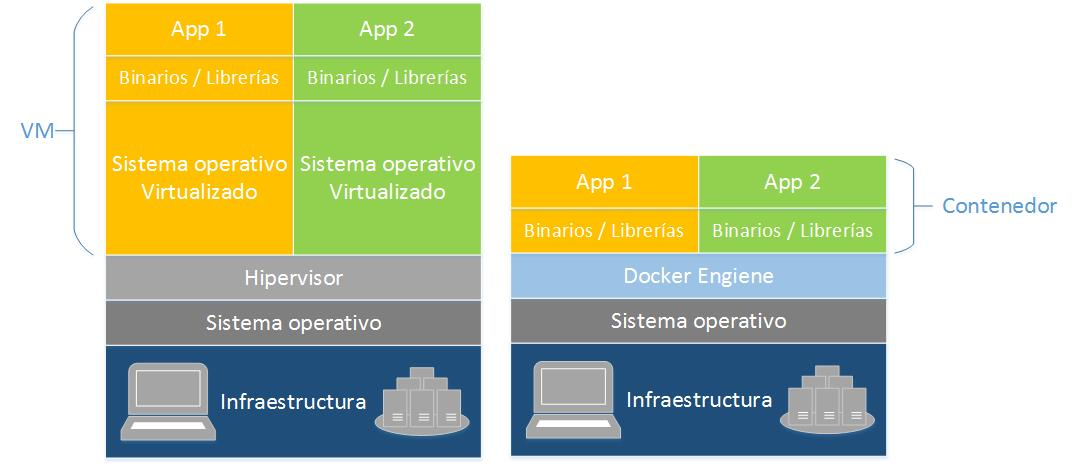
\includegraphics[width=0.45\textwidth]{./setup/VrvsDocker}
\caption{Comparativa de máquina virtual y Docker}
\label{Vs:VrvsDocker}
\end{center}
\end{figure}

En la figura \ref{Vs:VrvsDocker} se aprecian las diferencias comentadas anteriormente. La primera columna corresponde a la virtualización de 2 aplicaciones mediante la capa
intermedia del Hipervisor, el cual nos permite ejecutar los sistemas operativos virtualizados. Estos, a su vez, permiten ejecutar todos los binarios y librerías que requiere cada aplicación y, finalmente, la aplicación. La segunda columna corresponde a la contenerización de 2 aplicaciones mediante Docker Engine. Podemos observar
que no hace falta un hipervisor ya que utilizan el sistema operativo de la infraestructura
de donde son ejecutadas, pero sí son necesarios los binarios y las librerías. A simple vista se puede apreciar que, si eliminamos el sistema operativo, la infraestructura completa se hace más liviana y rápida de ejecutar.

\section{¿Por qué Docker?}\label{PqD:PQDocker}

Según lo listado en los apartados anteriores, se decidió utilizar Docker para realizar el despliegue de las aplicaciones por:

Cumplir con la condición de tecnología que pueda ser almacenada en dispositivos con una memoria reducida.

Su rapidez a la hora de levantar el servicio. En el mundo de IoT el tiempo es un bien
preciado y los sistemas se pueden apagar y encender constantemente para evitar gastos de energía innecesarios.

La facilidad para poder desplegar los servicios. Con Docker desplegar servicios es muy sencillo, solo requiere tenerlo instalado y ejecutar el contenedor para que el servicio esté activo.

La sencillez a la hora de mantener el sistema. Si hay que hacer actualizaciones o controles de una pequeña parte del servicio solo habría que cambiar o actualizar ese contenedor y no todo el sistema. Esto es un gran ahorro en recursos y tiempo. 

Por todos estos motivos se piensa que Docker puede ser una buena tecnología para desplegar sistemas de IoT. También hay que tener en cuenta que, aunque la Raspberry Pi no es un aparato con unas capacidades limitadas como podría ser un sensor utilizado normalmente, sí que cumple con todas las funciones listadas anteriormente y, por lo tanto, puede servir como preámbulo para la utilización en el resto de despliegues.  

\section{¿Cómo funciona Docker?}

En este punto se explicarán brevemente aspectos de la arquitectura, funcionamiento y
puesta en marcha de Docker.  

\subsection{Arquitectura}

Docker usa una arquitectura cliente-servidor. El cliente de Docker se comunica con el
Daemon de Docker para crear, ejecutar y distribuir los contenedores. Tanto el cliente como el Daemon pueden estar en el mismo sistema o pueden conectarse remotamente.
Como Docker usa el kernel de Linux para su ejecución, si el sistema operativo del sistema no es éste, se deberá usar una pequeña capa extra en la arquitectura de tipo VM (boot Docker) para poder correr Docker en la máquina.\newline

\subsubsection{Cliente de Docker}

Es la principal interfaz de usuario para Docker. Acepta los comandos del usuario y se
comunica con el Daemon de Docker.

\subsubsection{Imágenes de Docker (Docker Images)}

Las imágenes de Docker son plantillas de sólo lectura, que nos permitirán crear contenedores basados en su configuración.

\subsubsection{Registros de Docker (Docker Registries)}

Los registros de Docker guardan las imágenes. Éstos son repositorios públicos o privados donde se pueden subir o descargar imágenes. Sería similar a GitHub para imágenes de Docker (Docker Hub).

\subsubsection{Contenedores de Docker (Docker Containers)}

El contenedor de Docker contiene todo lo necesario para ejecutar una aplicación. Cada contenedor se crea de una imagen de Docker y es una plataforma aislada.
\newline

En la figura \ref{Inf:Infraestructura} podemos apreciar gráficamente cómo sería la arquitectura básica. El cliente podría hacer los comandos básicos de docker:

\texttt{Docker Build}: Hacer un build de un DockerFile y generar una imagen de Docker. En la figura está representado siguiendo las flechas rojas en las cuales podemos ver que el cliente se comunica con el Daemon y éste genera la imagen.

\texttt{Docker Pull}: Permite descargar una imagen de los repositorios de Docker. En la imagen se puede observar siguiendo las flechas verdes e, igual que el comando anterior, se comunica el cliente con el Daemon para que éste proceda a hacer la descarga de la imagen de mongoDB del repositorio. 

\texttt{Docker Run}: Ejecuta una imagen para generar un contendor de ésta. Siguiendo las flechas azules, veremos cómo nuevamente el cliente, al ejecutar esa comanda, se comunica con el Daemon. Este busca la imagen que se quiere ejecutar, en este caso la imagen de Ubuntu y se levanta un contenedor con la configuración de la imagen.
%\pagebreak 

\begin{figure}[htb]
\begin{center}
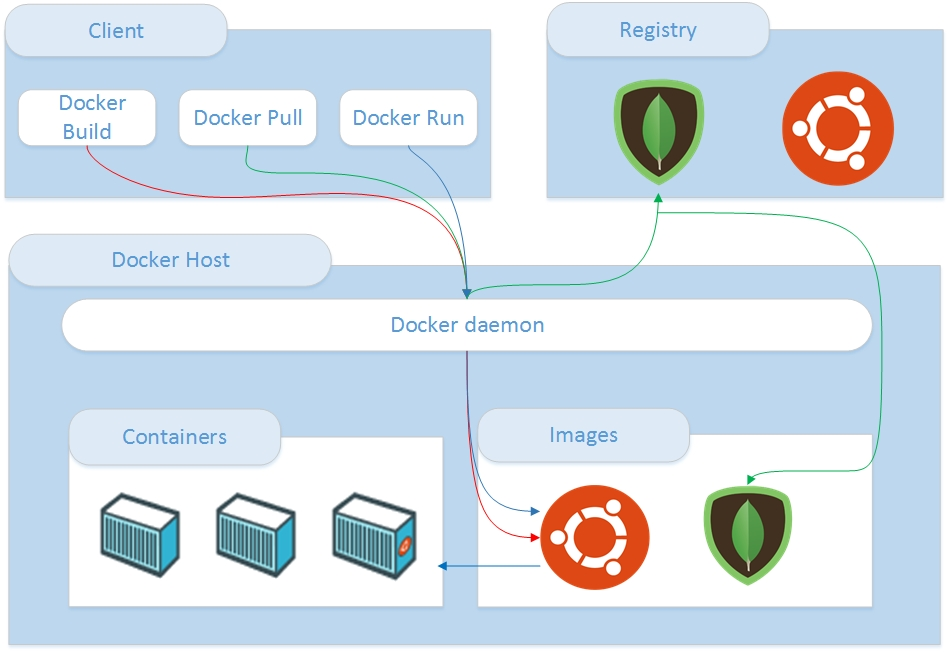
\includegraphics[width=0.69\textwidth]{./setup/Infraestructura}
\caption{Infraestructura de Docker}
\label{Inf:Infraestructura}
\end{center}
\end{figure}

\subsection{Creación de Imágenes}

Como se comenta en el punto anterior, las imágenes de Docker son las plantillas para
poder levantar los contenedores. Por eso la importancia de saber crear imágenes y personalizarlas ya que sólo permiten lectura y los cambios que hagamos en los contenedores no se verán reflejados en éstas.

La manera más sencilla de crear una imagen es descargarla del Docker Hub con el comando explicado anteriormente:

\begin{center}
\texttt{docker pull [OPTIONS] NAME[:TAG|@DIGEST]}
\end{center}

Este comando nos permite descargar una imagen en una versión concreta o tag dependiendo de nuestras necesidades. Por defecto, si no se pone nada, descargará la última. 

\begin{figure}[htb]
\begin{center}
\subfigure[Docker pull]{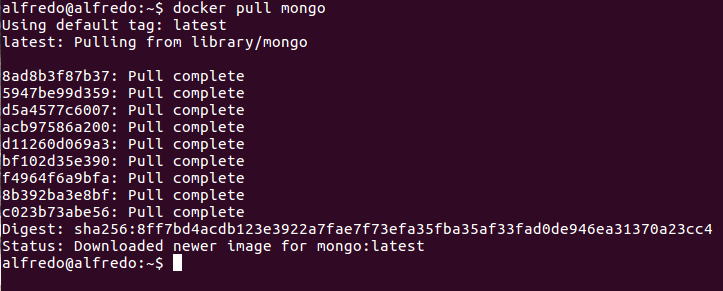
\includegraphics[width=0.90\textwidth]{./setup/DockerPull}}
\subfigure[Docker images]{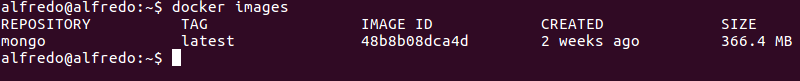
\includegraphics[width=0.90\textwidth]{./setup/DockerImages}}
\caption{Comandos de Docker (I)}
\label{Com1:ComandosDocker1}
\end{center}
\end{figure}

En la figuras \ref{Com1:ComandosDocker1} podemos apreciar como se descarga la última versión de la imagen de MongoDB y nos genera la imagen. 

Una vez obtenida la imagen se pasará a levantar el contenedor para poder ejecutar el servicio con otro de los comandos explicados. 

\begin{center}
\texttt{docker run [OPTIONS] IMAGE [COMMAND] [ARG...]}
\end{center}
\pagebreak 

\begin{figure}[htb]
\begin{center}
\subfigure[Docker ps]{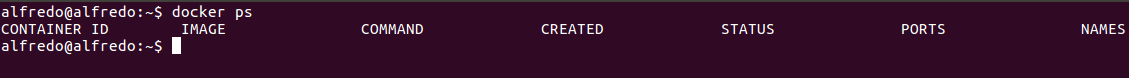
\includegraphics[width=0.90\textwidth]{./setup/DockerPs}}
\subfigure[Docker run]{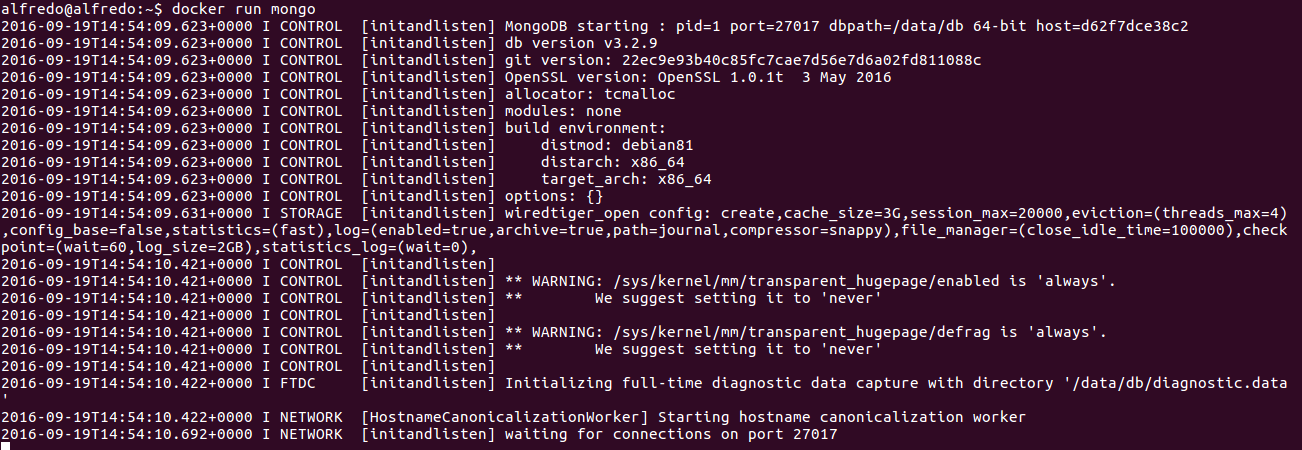
\includegraphics[width=0.90\textwidth]{./setup/DockerRun}}
\subfigure[Docker ps]{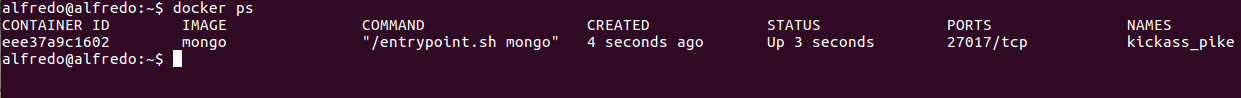
\includegraphics[width=0.90\textwidth]{./setup/DockerPsDespues}}
\caption{Comandos de Docker (II)}
\label{Com2:ComandosDocker2}
\end{center}
\end{figure}


En la figuras \ref{Com2:ComandosDocker2} se puede apreciar cómo utilizando el comando \texttt{docker ps} que
permite ver qué contenedores están levantados, no hay ninguno (a) y cómo al inicializar con el comando  \texttt{docker run mongo} levanta el servicio (b) y esta vez sí aparece el contenedor (c).

La segunda manera de crear y personalizar imágenes es mediante un \texttt{DockerFile}, que es un documento de texto donde se encuentran los comandos que se deben ejecutar para generar nuestra imagen.

El comando \texttt{docker build} comunica al Daemon de Docker que debe de leer el \texttt{DockerFile} del directorio actual y seguir las instrucciones línea por línea para la creación de nuestra imagen. Este proceso va pintando los resultados por pantalla y generando imágenes intermedias para obtener así una caché que nos permitirá en caso de errores, una vez corregido el DockerFile, continuar desde el punto conflictivo. 

\begin{verbatim}
FROM docker/whalesay:latest
CMD echo "Proyecto CoIoTe" | cowsay
\end{verbatim}

Aquí tenemos un ejemplo sencillo de DockerFile que nos servirá para explicar de una manera rápida como crearlos. 

\texttt{FROM} indica la imagen base que va a utilizar para seguir futuras instrucciones. Buscará si la imagen se encuentra localmente, en caso de que no, la descargará. En nuestro ejemplo utiliza la última versión de la imagen docker/whalesay.

La instrucción \texttt{CMD} solo puede aparecer una vez en un DockerFile, si colocamos más de uno, solo el último tendrá efecto. El objetivo de esta instrucción es proveer valores por defecto a un contenedor. Estos valores pueden incluir un ejecutable u omitir un ejecutable que en dado caso se debe especificar un punto de entrada o entrypoint en las instrucciones. En nuestro caso pintaremos un texto que se le pasara a la aplicación Cowsay.

Existen muchas más instrucciones, algunas de éstas serán explicadas más adelante cuando sea necesario su uso. 

Una vez ejecutado el comando \texttt{docker build -t docker-whale .} donde el \texttt{-t} nos permite darle nombre a la imagen y el \texttt{ .} encontrar el DockerFile para ser compilado, tal y como se ve en la Figura \ref{Build:BuildDockerFile}, descarga del repositorio la imagen ya que no la tenemos en local. Creará una imagen intermedia que nos proporciona la caché en caso de fallo, continuará con la siguiente orden creando una nueva imagen y borrando las anteriores hasta obtener la imagen definitiva. 
 
\begin{figure}[htb]
\begin{center}
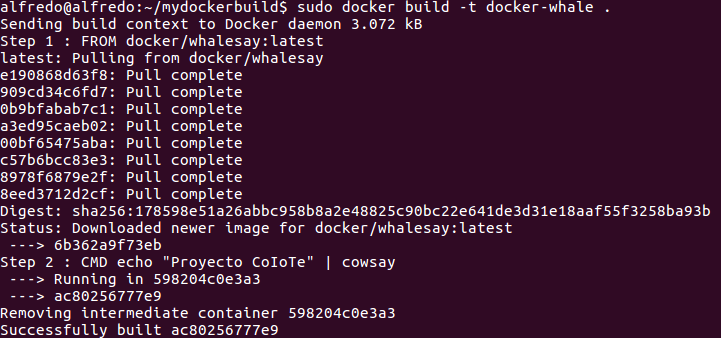
\includegraphics[width=0.90\textwidth]{./setup/DockerBuildWale}
\caption{Build del DockerFile}
\label{Build:BuildDockerFile}
\end{center}
\end{figure}
 
Una vez hecho el build del DockerFile podemos comprobar que nuestra imagen está creada correctamente (Figura \ref{Imag:ImageWhale}) y pasará a levantar el contenedor. Una vez levantado nos saldrá por pantalla el icono de Docker “diciendo” la frase que le indicamos en el fichero. (Figura \ref{Run:RunWhale}) 

\begin{figure}[htb]
\begin{center}
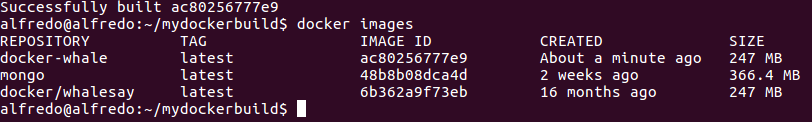
\includegraphics[width=0.90\textwidth]{./setup/DockerImagesWhale}
\caption{Docker images}
\label{Imag:ImageWhale}
\end{center}
\end{figure}
\pagebreak

\begin{figure}[htb]
\begin{center}
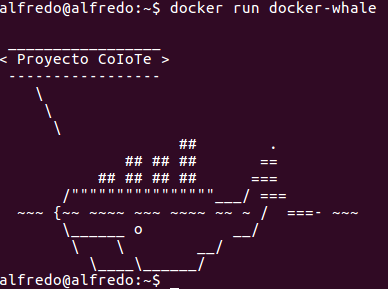
\includegraphics[width=0.70\textwidth]{./setup/DockerRunWhale}
\caption{Docker run docker-whale}
\label{Run:RunWhale}
\end{center}
\end{figure}

\subsection{Docker Compose}

Docker Compose es un orquestador que nos permite ejecutar aplicaciones que utilicen varios contenedores a la vez. Se creará un archivo docker-compose.yml donde se configurarán todos los servicios necesarios para nuestra aplicación. Una vez ejecutado este archivo nos generará todas las imágenes y con éstas los contenedores especificados a la vez que arrancará la aplicación.

Los comandos que se utilizarán serán similares a los utilizados en la creación de imágenes.

Para ejecutar el servicio y levantar todos los contenedores.

\begin{center}
\texttt{docker-compose up}
\end{center} 

Para detener el servicio y detener los contenedores.

\begin{center}
\texttt{docker-compose stop}
\end{center} 
%\pagebreak 

Docker-compose también permite ejecutar solo partes del.yml para levantar y/o detener solo algunos de los contenedores, pasándoles por parámetro el nombre del contenedor.

\begin{center}
\begin{verbatim}
version: '2'
services:
 mongo:
  container_name: mongo
  restart: always
  image: partlab/ubuntu-arm-mongodb
  volumes:
   - mongo-data:/data/db
  command: /usr/bin/mongod --smallfiles --journal
  \end{verbatim}
\begin{verbatim}
 aaaida:
  container_name: aaaidaArm
  restart: always
  image: alteraid/aaaida-datastore-arm
  links:
   - mongo:mongo 
  environment:
   - NODE_ENV=docker
  ports:
   - "40000:40000"
volumes:\newline
 mongo-data:
   driver: local
\end{verbatim}
\end{center}

Este es un ejemplo de Docker-compose, exactamente el utilizado en el proyecto para poder levantar la infraestructura de Aaaida en la Raspberry Pi. 
La importancia en los espacios es imprescindible para que éste funcione ya que da la jerarquía adecuada para que docker-compose lo entienda.
Ahora pasaremos a explicar brevemente los argumentos que podemos encontrar en él. 
En primer lugar tenemos los servicios, en nuestro caso son 2, una base de datos MongoDB y Aaaida.

Dentro de \texttt{mongo} tendremos los siguientes: 

\texttt{container name}: Le da un nombre al contenedor para no tener que referirse a él por la id o el nombre aleatorio que proporciona Docker.

\texttt{restart}: Nos permite que en caso de fallida o reinicio del sistema este contenedor vuelva a ejecutarse.

\texttt{image}: Para poder especificar la imagen que utilizaremos para este servicio.

\texttt{volumes}: En caso de Mongo necesita un directorio donde almacenar los datos. Ésto especıfica donde se creará el volumen de datos.

\texttt{command}:  El comando que le pasamos al contenedor al momento de su ejecución. En este caso concreto es muy importante ejecutar este comando ya que activará el Journaling, que por defecto viene desactivado.

En el siguiente servicio, el de \texttt{aaaida}, a parte de disponer los mismos argumentos basicos como serian \texttt{container name}, \texttt{restart} o \texttt{image}, encontraremos alguno más como:

\texttt{links}: Define el enlace entre contenedores.

\texttt{environment}: Para poder poder pasar variables.

\texttt{ports}: Define el mapeo de puertos.

Para finalizar el archivo se encuentra los \texttt{volumes} donde se genera el volumen que hemos especificado dentro del servicio de \texttt{mongo}.  

En puntos posteriores se explicará más detenidamente el funcionamiento y la puesta en marcha del Docker Compose ya que el archivo utilizado para el ejemplo es el utilizado en la Raspberry.

\section{Conclusiones}

Como se puede observar, al virtualizar los recursos disponibles obtenemos un aumento en rendimiento y una reducción de los costes. 

Docker nos permite el despliegue de aplicaciones de una manera sencilla y en cualquier plataforma que lo soporte. 

La diferencia más significativa entre las máquinas virtuales y Docker sería el uso del Hipervisor y la necesidad de un sistema operativo para las máquinas virtuales, cosa que en Docker no es necesario. Ésto hace que las aplicaciones desplegadas de esta manera tengan una reducción en tamaño y en tiempo de ejecución.

\chapter{Raspberry Pi}

\section{¿Por qué Raspberry Pi?}

Los motivos por los cuales se ha utilizado una Raspberry Pi en este proyecto son claros y han sido comentados con anterioridad. Es un dispositivo portátil de un tamaño muy reducido que nos facilita mucho el poder llevarlo y poder ofrecer un servicio en cualquier lugar sin dificultades. Tiene unas prestaciones más que aceptables para un dispositivo de ese tamaño como conexiones inalámbricas de Wifi y Bluetooth integrados, cosa imprescindible para las comunicaciones con los sensores. Todo a un precio muy atractivo que lo hace asequible.  

Algunas de las especificaciones mas importantes de las Raspberry Pi 3 son las siguientes:
\begin{itemize}
\item 1.2GHz 64-bit quad-core ARMv8 CPU
\item 802.11n Wireless LAN
\item Bluetooth 4.1 y Bluetooth Low Energy (BLE)
\item 1GB RAM
\item Ethernet port
\item Micro SD card slot 
\end{itemize}

\begin{figure}[htb]
\begin{center}
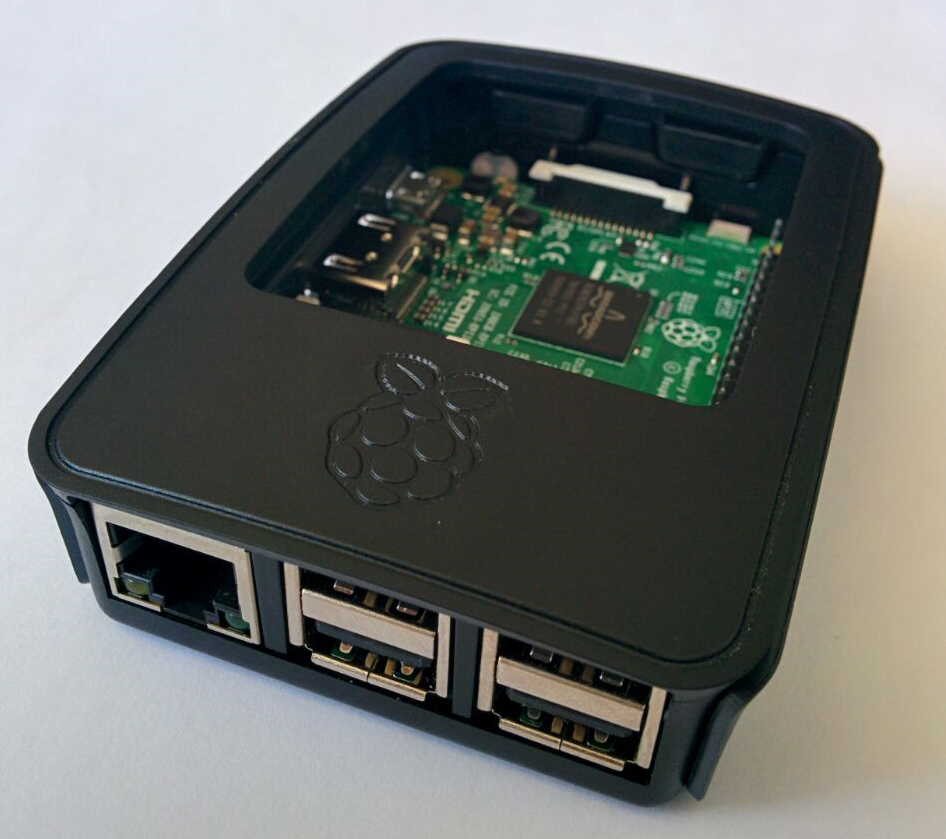
\includegraphics[width=0.65\textwidth]{./setup/raspi}
\caption{Raspberry Pi 3}
\end{center}
\end{figure}


\section{Virtualización de la Raspberry Pi}

Al inicio del proyecto no se disponía de una Raspberry Pi para poder realizar las pruebas y se decidió emularla mediante Qemu. 
Qemu es una aplicación que nos permite emular, mediante máquinas virtuales, gran parte de los sistemas operativos. 
Es realmente sencillo emular una imagen de Raspbian Pi si no fuera por un detalle, como se comenta en el apartado 2.2: ¿Qué es Docker? Docker necesita un sistema x64 o Linux kernel 3.8+ mientras que Raspberry Pi ejecuta un sistema ARM, lo que conlleva que Docker no sea compatible a primera instancia con la Raspberry Pi. 
La solución para este gran problema es la utilización de Hypriot, una imagen de Raspbian modificada con Docker instalado. 
La instalación de esta imagen requiere hacer unos retoques ya que el kernel de Qemu no es del todo compatible con el de la imagen de Hypriot. Desafortunadamente, las incompatibilidades del kernel no permitían hacer un uso correcto de modo que se decidió apartar por completo la posibilidad de poder emular una Raspberry Pi con Docker instalado ya que las incompatibilidades del kernel no lo permitían.

En el apéndice se podrán ver los pasos a seguir para la instalación y emulación de la imagen. 

\section{Raspberry Pi y Docker}

Después de descartar completamente la opción de emular la imagen en Qemu se decidió probar en la Raspberry Pi de la empresa si la imagen corría correctamente. Y sí, la imagen iba perfectamente y ejecutaba Docker sin ningún problema. Contrariamente, la Raspberry Pi sí que dio problemas porque era el primer modelo, que era antiguo, y no disponía de módulos para conexiones inalámbricas integrados por lo que se decidió, aprovechando el lanzamiento de la nueva Raspberry Pi 3, comprarla ya que ésta sí dispone de de conexiones inalámbrica. 

\subsection{Instalación de la imagen en la Raspberry Pi}

Como se ha dicho, a la imagen de Raspbian no es posible instalar Docker como lo haríamos en un sistema operativo como linux. Es necesario una imagen la cual ya lo tenga instalado, como la imagen de Hypriot. La instalación se llevó a cabo de esta manera:

\begin{verbatim}
$ curl -sSL http://downloads.hypriot.com/docker-hypriot_1.8.2-1_armhf.deb 
>/tmp/docker-hypriot_1.8.2-1_armhf.deb
$ sudo dpkg -i /tmp/docker-hypriot_1.8.2-1_armhf.deb
$ rm -f /tmp/docker-hypriot_1.8.2-1_armhf.deb
$ sudo sh -c 'usermod -aG docker $SUDO_USER'
$ sudo systemctl enable docker.service
\end{verbatim}

\begin{itemize}
\item Primero descargá la imagen deseada y la montará en un directorio temporal.
\item Instalará los paquetes con el comando dpkg.
\item Borrará el archivo comprimido.
\item Ejecutará el comando donde añade el usuario a un grupo Docker. 
\item Pondrá en marcha el Daemon de Docker.  
\end{itemize}


\subsection{Creación de las imágenes de Docker}

Una vez tenemos la Raspberry lista, se pasará a la creación de las imágenes Docker para poder desplegar Aaaida.
En primer lugar se necesita un contenedor que contenga una base de datos, en este caso MongoDB. Para la creación de la imagen utilizaremos una ya creada y que esté en los repositorios de Docker Hub. Se necesita una imagen que sea compatible con ARM, cosa que no resulta sencillo ya que la gran mayoría de las imágenes no están pensadas para esta arquitectura y los pocos disponibles no estaban operativos. Otra restricción que tenemos era que debe ser una base de datos sin la necesidad de ingresar un usuario y su contraseña, cosa que no es habitual, pero que resulta una obligación en algunas imágenes.
Por lo tanto se utilizó la siguiente imagen de Docker Hub:

\begin{center}
\texttt{partlab/ubuntu-arm-mongodb}
\end{center}

La otra imagen que se utilizará será la propia de Aaaida, pero igual que, la imagen de MongoDB deberá ser compatible con una arquitectura ARM. Al ser una aplicación propia de la empresa no se encontrará en repositorios público y tendremos que crearla nosotros mediante un Dockerfile. 
En la siguiente figura se puede ver el Dockerfile que se utilizará para poder crear el contenedor con Aaaida.

\begin{verbatim}
FROM ioft/armhf-debian
RUN apt-get update; apt-get -y install curl
RUN set -ex \  
	&& for key in \    
		9554F04D7259F04124DE6B476D5A82AC7E37093B \ 
        94AE36675C464D64BAFA68DD7434390BDBE9B9C5 \
        0034A06D9D9B0064CE8ADF6BF1747F4AD2306D93 \ 
        FD3A5288F042B6850C66B31F09FE44734EB7990E \    
        71DCFD284A79C3B38668286BC97EC7A07EDE3FC1 \    
        DD8F2338BAE7501E3DD5AC78C273792F7D83545D \    
        B9AE9905FFD7803F25714661B63B535A4C206CA9 \    
        C4F0DFFF4E8C1A8236409D08E73BC641CC11F4C8 \  
	; 	do \  
		gpg --keyserver ha.pool.sks-keyservers.net --recv-keys "$key"; \  
	done

ENV NODE_VERSION 4.4.5

RUN curl -SLO 
"https://nodejs.org/dist/v$NODE_VERSION/node-v$NODE_VERSION-
linux-armv7l.tar.gz" \  
&& curl -SLO "https://nodejs.org/dist/v$NODE_VERSION/SHASUMS256.txt.asc" \  
&& gpg --batch --decrypt --output SHASUMS256.txt SHASUMS256.txt.asc \  
&& grep "node-v$NODE_VERSION-linux-armv7l.tar.gz\$" SHASUMS256.txt | 
sha256sum -c - \  
&& tar -xzf "node-v$NODE_VERSION-linux-armv7l.tar.gz" -C /usr/local 
--strip-components=1 \  
&& rm "node-v$NODE_VERSION-linux-armv7l.tar.gz" SHASUMS256.txt.asc 
SHASUMS256.txt

COPY scripts/rpi_docker/entrypoint /entrypoint
RUN mkdir /aaaida
WORKDIR /aaaida
CMD ["/entrypoint"]
EXPOSE 40000
COPY . /aaaida
\end{verbatim}

Al principio del Dockerfile se ve la acción \texttt{FROM}, encargada de cargar una imagen de una Debian para ARM. Como observación se puede detectar que la imagen del mongo es para Ubuntu ARM y la imagen base para Aaaida es una Debian ARM, distribuciones de linux diferentes en los dos contenedores. Esto demuestra que cada contenedor es un ente aislado que no tiene que depender del resto de contenedores.
 
A continuación de declarar la imagen base, vienen una serie de acciones con la instrucción \texttt{RUN}, que nos permite ejecutar cualquier comando. En el primer caso que hace un update e instala el curl.
 
Las siguientes tres instrucciones de las cuales dos de ellas son un \texttt{RUN} y la restante un \texttt{ENV}, que configura las variables de entorno, son para poder instalar el Node.js en el contenedor para poder compilar el código de Aaaida.
 
Una vez instalado se utiliza la acción \texttt{COPY}, que como su nombre indica, copiara el contenido de un directorio en un directorio del contenedor.

Si seguimos se ve que crea un directorio con el nombre de \texttt{aaaida} y hace que ese directorio sea el directorio de trabajo con la instrucción \texttt{WORKDIR}.
 
Después Ejecutará \texttt{[/entrypoint]} que al escribirlo en formato JSON la instrucción \texttt{CMD} ejecuta el contenido sin shell. El contenido de este script especifica los puertos, el host... de la aplicación. Se podrá ver su contenido en el apéndice.
 
Para terminar con las 2 últimas instrucciones, que son \texttt{EXPOSE} y \texttt{COPY}, la cual la primera indica los puertos que el contenedor tendrá activos y por los cuales escuchará. El segundo hará una copia desde el punto raíz donde se ejecutará el Dockerfile en el directorio creado anteriormente de \texttt{aaaida}.

\subsection{Despliegue de la aplicación} 

Para realizar el despliegue de Aaaida, con las dos imágenes que se han creado en el apartado anterior será suficiente. Tan solo tendremos que arrancar las imágenes para crear los contenedores. 
Primero se hará un \texttt{docker run} sobre la imagen de MongoDB y acto seguido igual con la imagen de Aaaida, pero con una pequeña diferencia: habrá que linkear el contenedor de mongo para que la aplicación pueda encontrar la base de datos necesaria para funcionar.
\pagebreak 

El comando utilizado para levantar el contenedor sería el siguiente:

\begin{center}
\begin{verbatim}
docker run --link=cc1d12ed96ee:mongo --name= aaaidaArm -e NODE_ENV=docker 
alteraid/aaaida datastore-arm
\end{verbatim}
\end{center}

En el comando se linkea el \texttt{CONTAINER ID} que sería como el número de serie del contenedor de Docker (se puede obtener usando el comando \texttt{docker ps}), también le dará un nombre al contenedor y por último el -e que permite añadir variables de entorno.
\newline 

Pero levantar los contenedores utilizando solo Docker implica estar haciendo un \texttt{run} o \texttt{start} cada vez que el servicio caiga por culpa de un apagón o fallos. Se decide instalar Docker Compose para poder orquestar las dos imágenes y añadir todas las necesidades y relaciones que necesiten. Esto permitirá tener el servicio automatizado en un fichero que tan solo habrá que arrancar una vez y en caso de fallo, el solo intentara arrancar de nuevo el servicio. El fichero utilizado se puede ver en el punto 2.5.3. Docker Compose donde también está explicado. 

Si se levanta el proceso mediante el comando \texttt{docker-compose up} se puede ver como tanto el contenedor de \texttt{aaaida} como el de \texttt{mongo} se ejecutan y tenemos la aplicación corriendo perfectamente.

\begin{figure}[htb]
\begin{center}
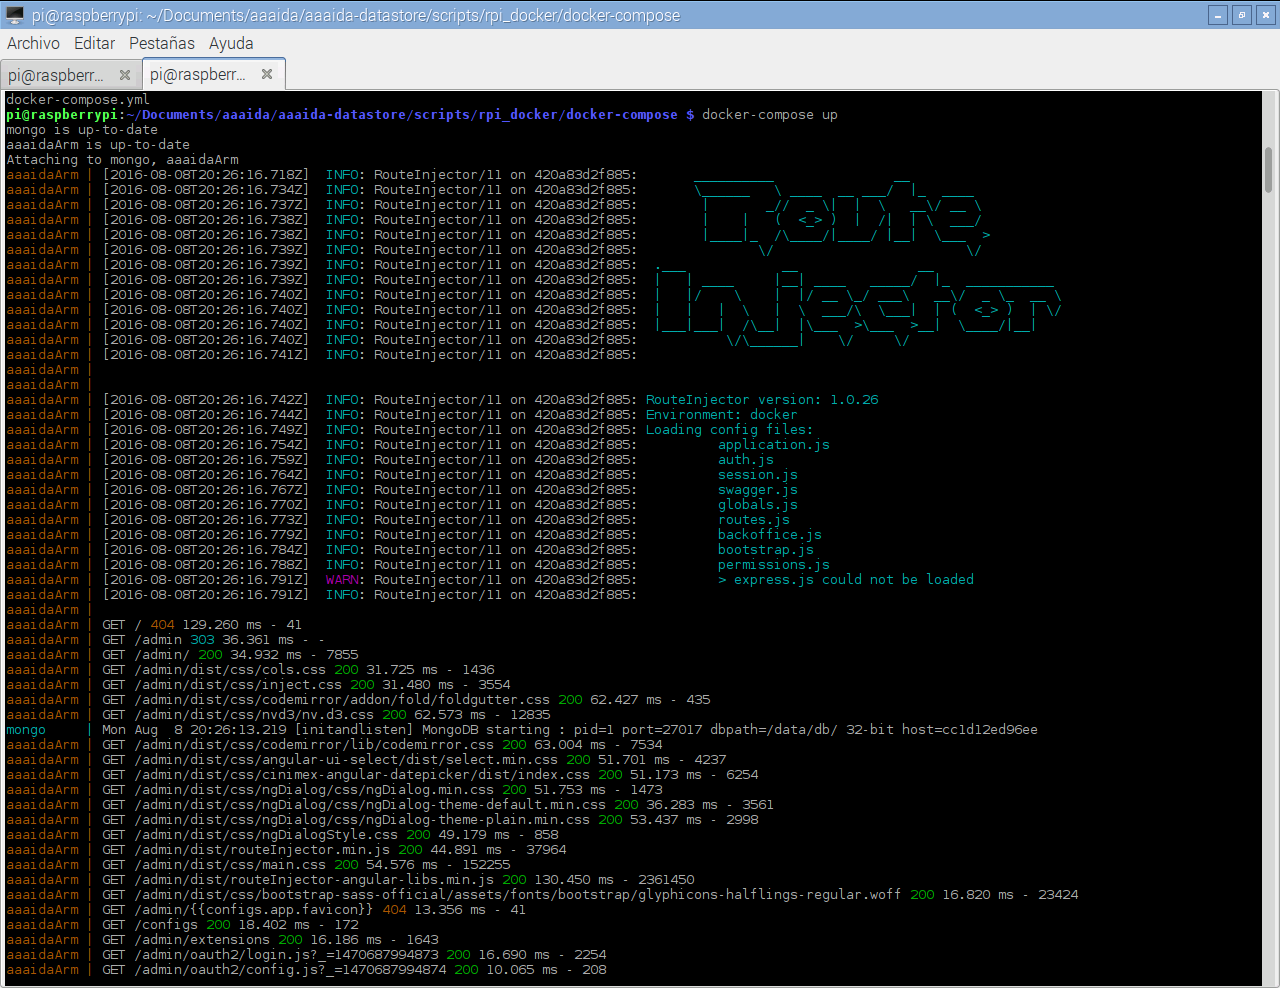
\includegraphics[width=0.95\textwidth]{./setup/dockerComposeUp}
\caption{Docker-compose up}
\label{ComUp:composeUp}
\end{center}
\end{figure} 
\pagebreak

\begin{figure}[htb]
\begin{center}
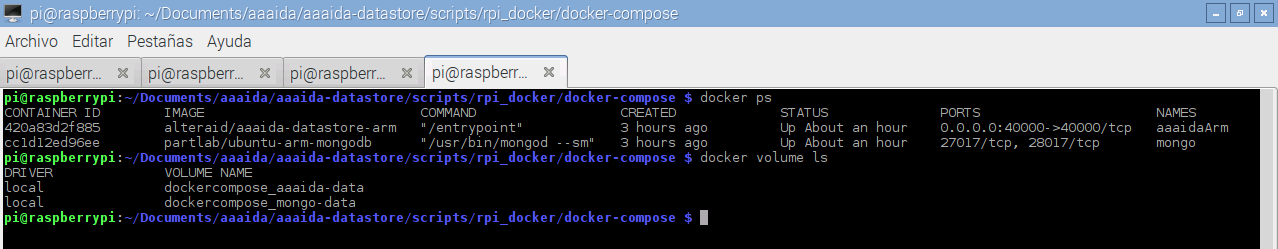
\includegraphics[width=0.95\textwidth]{./setup/dockerpsVolumen}
\caption{Listado de contenedores y volúmenes}
\label{psVl:psVolumen}
\end{center}
\end{figure} 

En las dos figuras anteriores (\ref{ComUp:composeUp} y \ref{psVl:psVolumen}) se puede ver cómo al iniciar el Docker Compose se levantan todos los contenedores y se crean los volúmenes de datos necesarios para arrancar la Aaaida, la cual si abrimos un navegador podremos acceder. (Figura \ref{webLog:LoggeoAaaida}) 

\begin{figure}[htb]
\begin{center}
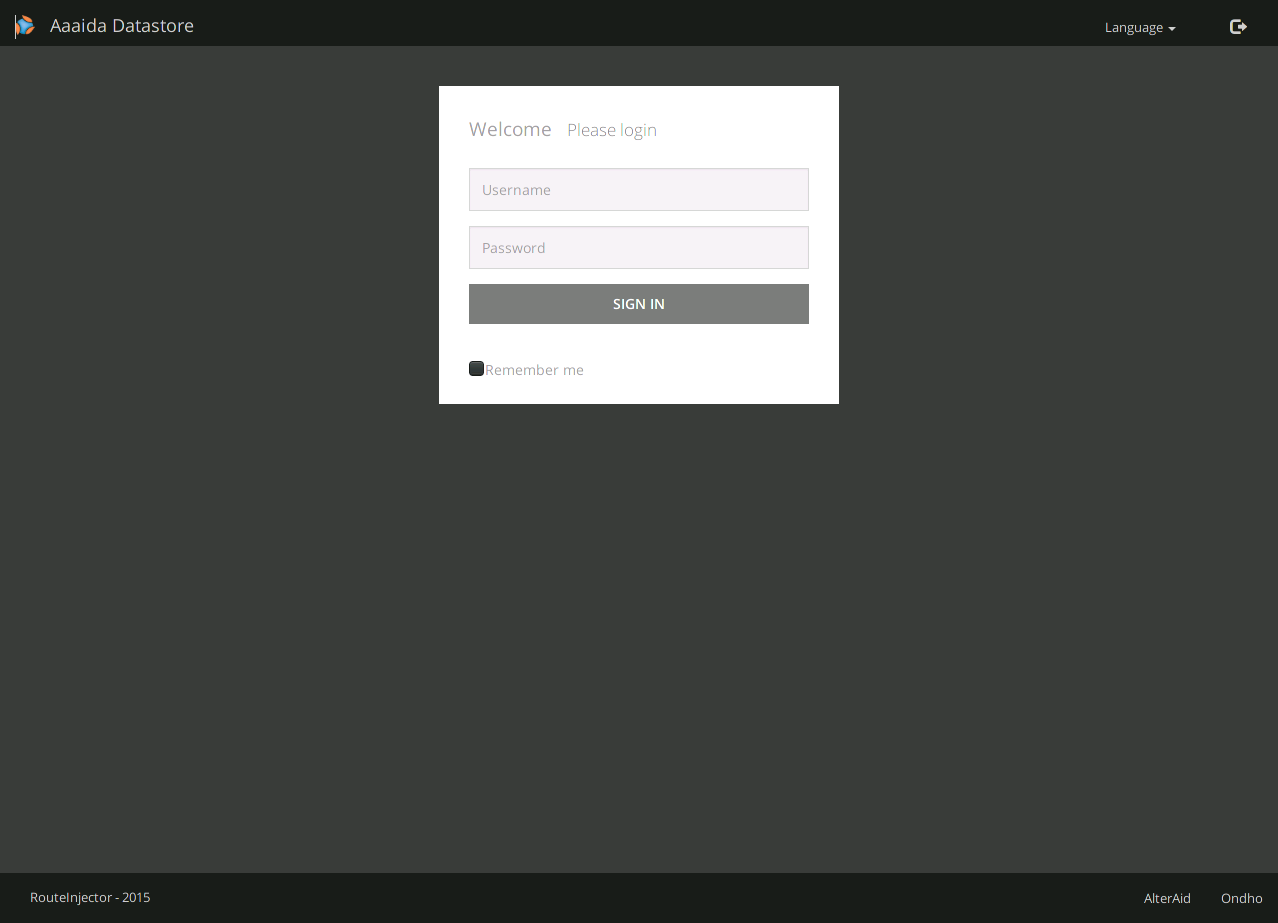
\includegraphics[width=0.95\textwidth]{./setup/AaaidaDatastore}
\caption{Acceso a Aaaida}
\label{webLog:LoggeoAaaida}
\end{center}
\end{figure} 

La base de datos está vacía. Al no tener datos no hay usuarios por lo tanto  no se podrá acceder a la plataforma de Aaaida, la solución es cargar un dump de la base de datos en el contenedor de \texttt{mongo} para que éste encuentre los datos y poder acceder a la plataforma.  Para hacer el volcado de datos es necesario saber la IP del contenedor ya que será la manera de decir donde queremos hacer el restore de la base de datos. Para poder extraer información de los contenedores se utiliza el comando \texttt{docker inspect}. En la figura siguiente se verá la ejecución del comando y de donde obtendremos la IP de nuestro contenedor de mongo.
\pagebreak

\begin{figure}[htb]
\begin{center}
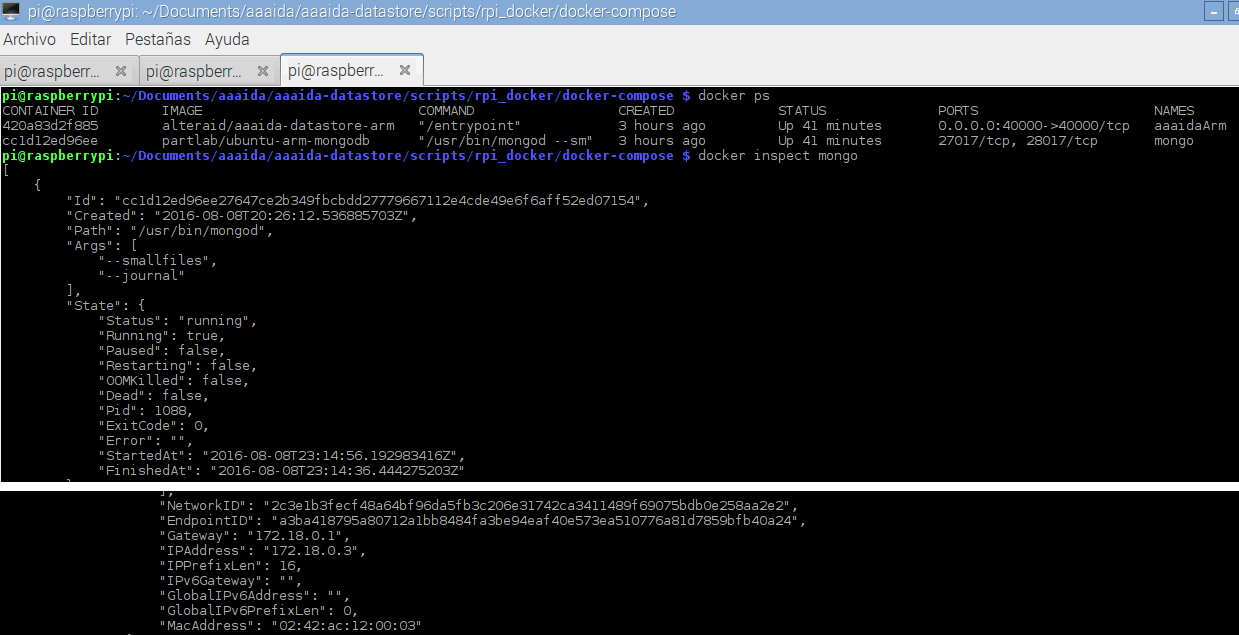
\includegraphics[width=0.95\textwidth]{./setup/dockerinspect}
\caption{Docker inspect}
\label{insp:dockerInspect}
\end{center}
\end{figure} 

Una vez se obtiene la IP del contenedor, \texttt{IPAddress: 172.18.0.3}, se ejecuta el siguiente comando para llevar a cabo el volcado de datos:

\begin{center}
\texttt{mongorestore dump/ -h 172.18.0.3}
\end{center}

Una vez disponemos de todas las piezas listas, se puede dar por concluido el proceso de despliegue de Aaaida en una Raspberry Pi utilizando Docker. 

\begin{figure}[htb]
\begin{center}
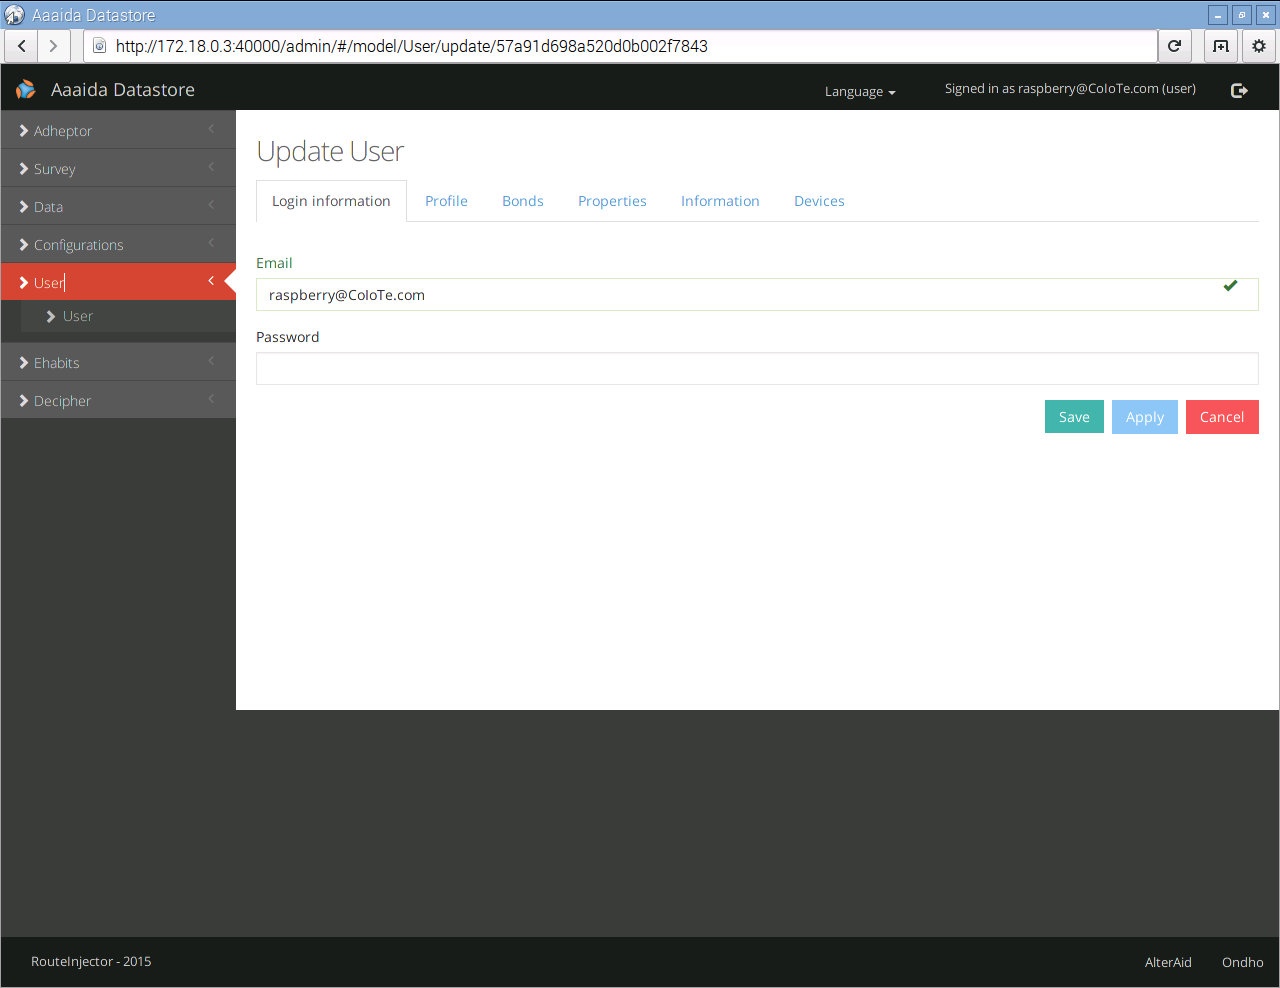
\includegraphics[width=0.70\textwidth]{./setup/aaaidaCoIoTe}
\caption{Interfaz de Aaaida}
\label{aidaCoI:aaaidaCoiote}
\end{center}
\end{figure} 
 
 \subsection{Conclusiones} 
 
En este capítulo se puede ver que la Raspberry Pi es el dispositivo para IoT más popular en el mercado, tanto por su prestaciones como por su reducido precio.
 
No es posible virtualizar la Raspberry Pi mediante Qemu y utilizar Docker ya que el kernel no es compatible. 

Y por último, aunque Docker no sea compatible para un sistema ARM gracias a unos pequeños cambios en la imagen sí puede ejecutar. Por lo tanto se pudo desplegar toda la infraestructura en la Raspberry Pi y Aaaida funciona perfectamente. 
\chapter{Aaaida}
\chapter{Implementación}

En este capítulo se explicará las implementaciones realizadas para poder llevar a cabo el proyecto, tanto como para conseguir la comunicación con el sensor, los cambios realizados en Aaaida para poder visualizar las mediciones del sensor y por último el despliegue en la Raspberry Pi. 

\section{Comunicación con el sensor}

Para la realización del proyecto es necesario un sensor que se pueda comunicar y enviar los datos mediante bluetooth. En la empresa se dispone de una serie de sensores médicos de los cuales se utilizará un monitor de ritmo cardiaco, Zephyr BioHarness 3. 

\begin{figure}[htb]
\begin{center}
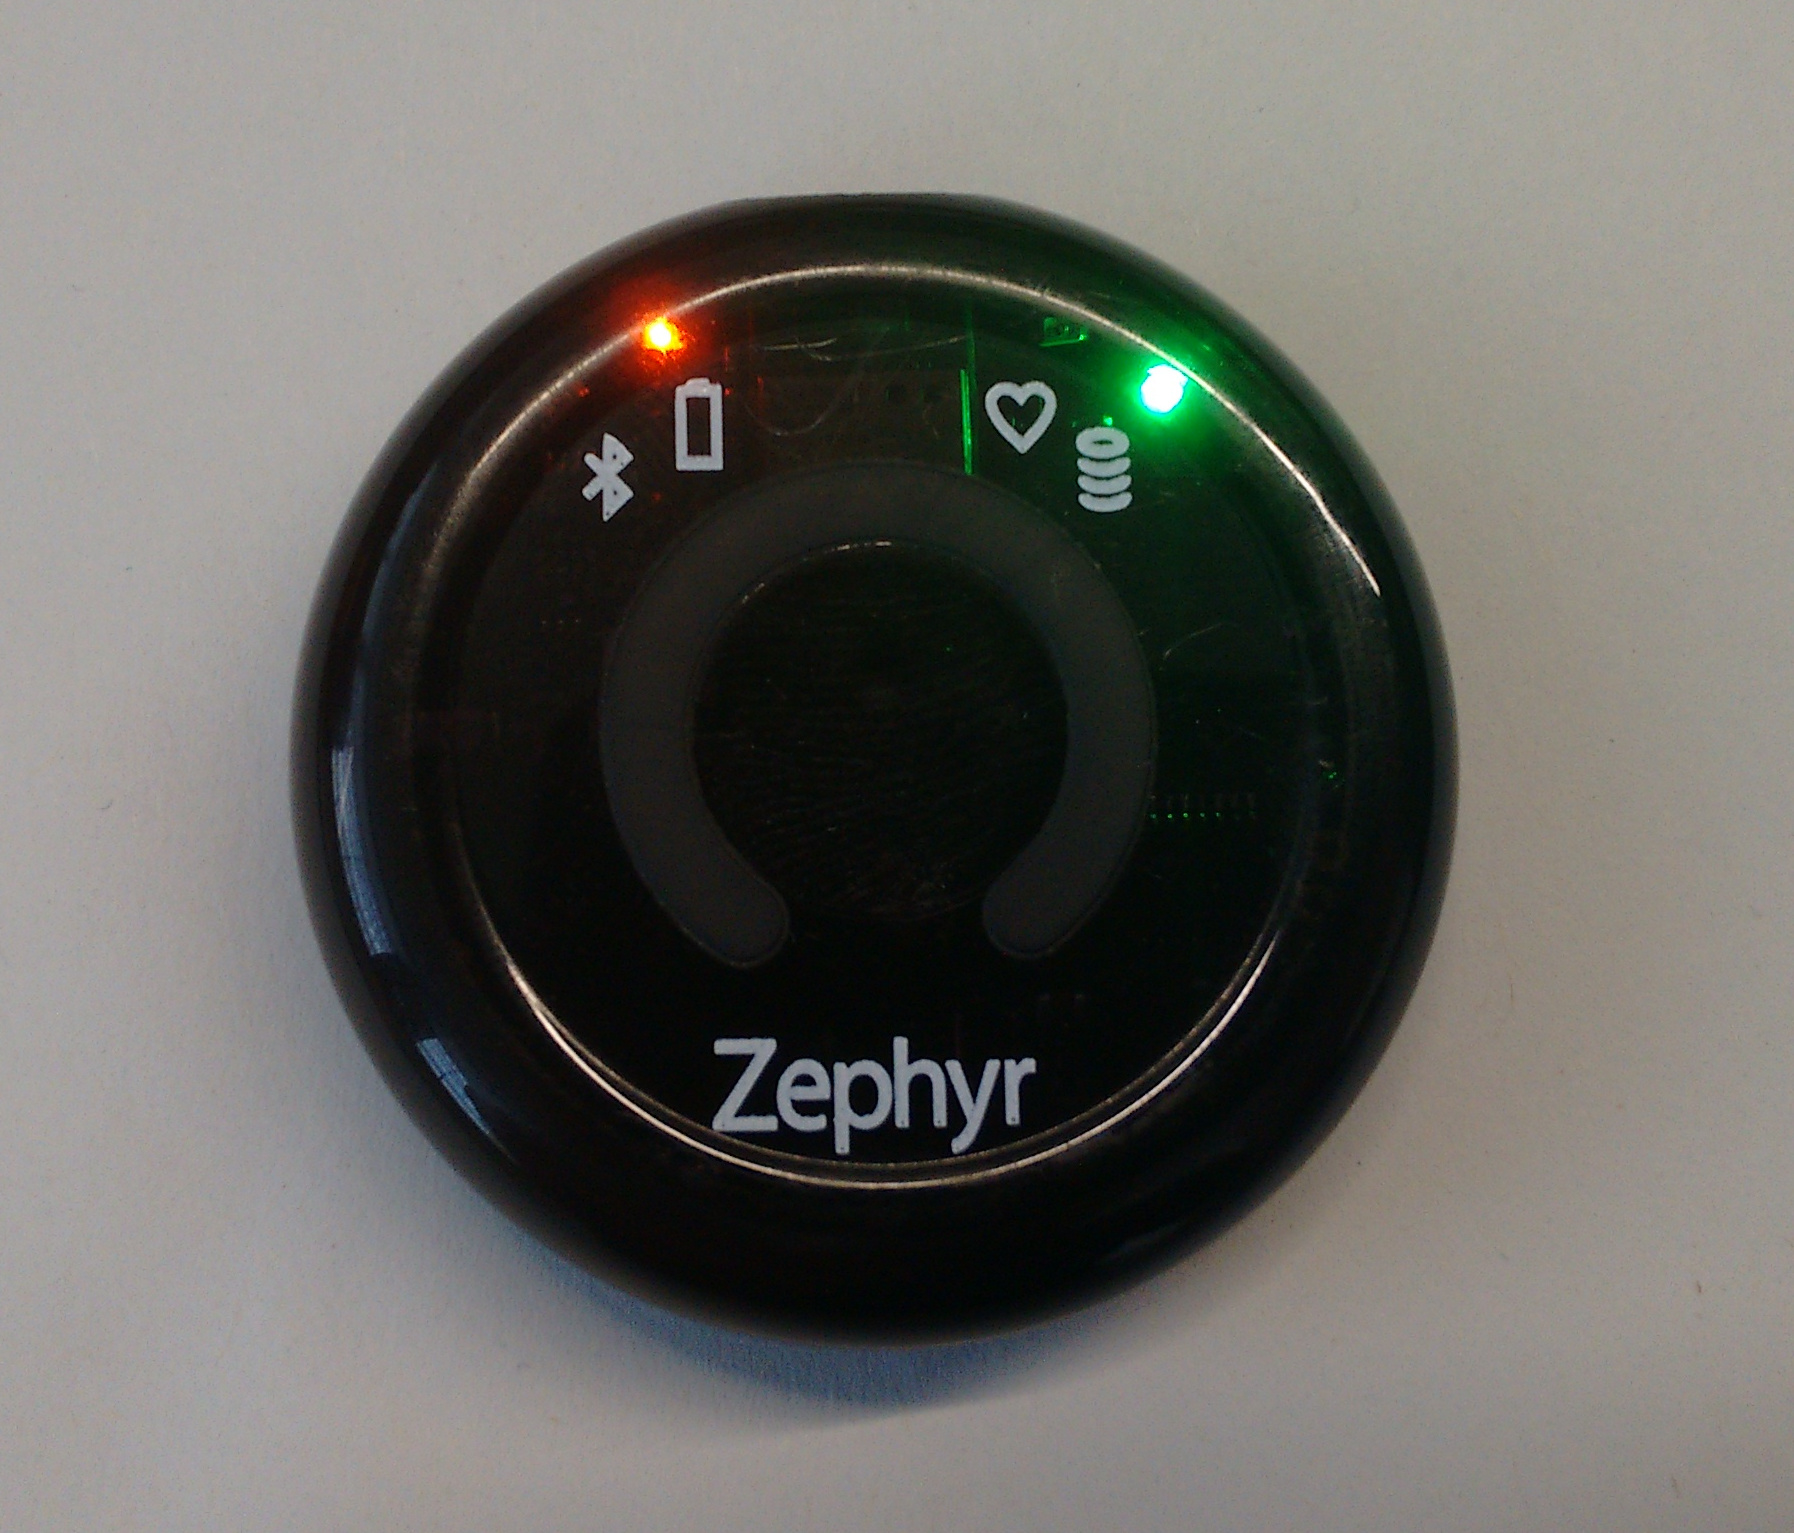
\includegraphics[width=0.5\textwidth]{./setup/zephyr}
\caption{Sesor Zephyr BioHarness 3}
%\label{a:arquitectura}
\end{center}
\end{figure}

El fabricante te ofrece gran cantidad de documentación y una aplicación de prueba para los desarrolladores que quieran realizar productos y utilicen sus sensores. Pero todo está orientado a aplicaciones Android, las cuales son las más populares para este tipo de sensores. 

Por lo tanto, después de buscar y ponerse en contacto con la empresa, no hay ningún tipo protocolo para establecer contacto y recibir los datos en JavaScript. Por lo que se decidió realizar uno utilizando toda la documentación y ejemplos para otros lenguajes. 

Para la realización del código de comunicación fueron necesarios 2 módulos de Node.js uno que nos calcula el CRC y otro que establece una conexión bluetooth.

Módulos utilizados:

\begin{itemize}
\item crc
\item bluetooth-serial-port 
\end{itemize}
\pagebreak

\subsection{Protocolo}

El código realizado para poder establecer la comunicaciones fue el siguiente:
 
Se cargan los módulos externos y se declaran las variables, la dirección MAC del sensor se pone a clavo para evitar interferencias con otros dispositivos bluetooth.

\begin{verbatim}
var crc = require('crc');
var btSerial = new (require('bluetooth-serial-port')).BluetoothSerialPort();

ADDRESS = "E0:D7:BA:A7:F1:5D";
var results = [];
var is_stopping = false;
\end{verbatim}

Función \texttt{connect}, como su nombre indica, nos conectara con el sensor y empezará a recibir datos. 

\begin{verbatim}
function connect(callback) {
   var socket = btSerial.on('found', function (address) {
       if (address == ADDRESS) {
           btSerial.findSerialPortChannel(address, function (channel) {
               btSerial.connect(address, channel, function () {
                   console.log('connected to ' + address);
                   btSerial.on('data', function (buffer) {
                       decode(buffer);
                   });
                   listener(socket, function (res) {
                       callback(res);
                   });
               }, function () {
                   console.log('cannot connect');
               });
           }, function () {
               console.log('found nothing');
           });
       }
   });
   btSerial.inquire();
}
\end{verbatim}

La función \texttt{decode}, nos permite decodificar de una manera muy simplificada los bytes que se reciben. Le pasa el segundo byte y según su valor se puede saber qué tipo de mensaje envía el sensor. Si en el segundo byte que se recibe es un 44 implica que en el noveno byte que se está recibiendo el ritmo cardiaco.

\begin{verbatim}
function decode(data) {
   switch (data[1]) {
       case 35:
           console.log("Received LifeSign message");
           break;
           \end{verbatim}
           %\pagebreak
           \begin{verbatim}
       case 44:
           console.log("Received Event message");
           results.push(data[8]);
           break;
       case 43:
           console.log("Received Summary Data Packet");
           break;
       case 37:
           console.log("Received Accelerometer Data Packet");
           break;
       case 36:
           console.log("Received R to R Data Packet");
           break;
       case 33:
           console.log("Received Breathing Data Packet");
           break;
       default:
           console.log("Packet type: " + data[1]);
           console.log("Received Not recognised message");
           break;
   }
}
\end{verbatim}

Una vez conectados al sensor se debe enviar mensajes a este para que mantenga la conexión y no se desconecte (\texttt{lifeSings}). Como la finalidad es realizar una medida la comunicación se realizará durante 20 seg, una vez pasados estos 20 seg se cerrara la conexion. 

\begin{verbatim}
function listener(socket, callback) {
   socket.on('data', function (buffer) {
       decode(buffer);
       lifeSing = create_message_frame('100011', 0);
       socket.write(new Buffer(lifeSing), function (err, bytesWritten) {
           if (err) console.log(err);
       });
   });
   setTimeout(function () {
       stop(socket, function (res) {
           callback(res);
       });
   }, 20000);
}
\end{verbatim}

La creación de los mensajes \texttt{lifeSings} se realizan de la siguiente manera: Son la concatenación de un byte de sincronismo, el mensaje, el dlc que será la longitud del payload, el crc calculado mediante el payload y por ultimo otro byte de cierre. Todo el paquete se pasará a hexadecimal y se procederá a enviarlo.
 \pagebreak
\begin{verbatim}
function create_message_frame(message_id, payload) {
   dlc = payload.toString().length;
   if (0 <= dlc <= 128) {
       crc_byte = crc.crc32(payload);
       message_bytes = '00000010'+ message_id + dlc + payload + crc_byte 
       + '00000011';
       message_fame = Bin2Hex(message_bytes);
       return message_fame
   }
}
\end{verbatim}

Por último la función de \texttt{stop} y la función de \texttt{avg}, la función de \texttt{stop} cerrará la conexión y la función de \texttt{avg} calcula la media de todas las medidas tomadas durante los 20 seg y devolverá la media. 

\begin{verbatim}
function stop(socket, callback) {
   is_stopping = true;
   socket.close();
   avg(function (res) {
       callback(res);
   });

}

function avg(callback) {
   var sum = 0;
   if (is_stopping == true) {
       for (var i = 0; i < results.length; i++) {
           sum = sum + results[i];
       }
       var media = sum / results.length;
       callback(media);
   }
}
\end{verbatim}

Con esto se puede establecer una conexión con el sensor y poder recibir la media del pulso cardiaco durante 20 seg. Hay que tener en cuenta la simplicidad del protocolo, ya que solo se captura una de las funciones (ritmo cardíaco) que proporciona el sensor Zephyr, ya que si se quiere obtener todos los datos la complejidad sería mucho mayor y para desarrollarlo en JavaScript se necesitaría mucha más información sobre cómo se envían las tramas y que contiene cada una de ellas.
\pagebreak
\section{Integración con Aaaida}

Como se explicó en el capítulo anterior la consola de Aaaida es una plataforma web, que nos permite administrar toda la información de las aplicaciones vinculadas a ella. 
Para poder incluir nuestra aplicación de monitorización del ritmo cardiaco con Aaaida y así visualizar lo en la web hay que crear un plugin de Aaaida con nuestro proyecto. 

\subsection{Creación de un plugin}

Para el desarrollo de cada uno de los plugins se ha utilizado el framework llamado route-injector desarrollado por Alteraid y Ondho. 

El objetivo principal de este framework es el de generar, de manera automática:
los método http CRUD de la API REST (GET, PUT, POST,DELETE) y una
backoffice, mediante modelos.

Para la creación del plugin de proyecto deberemos de seguir la arquitectura principal de los plugins.


\begin{figure}[htb]
\begin{center}
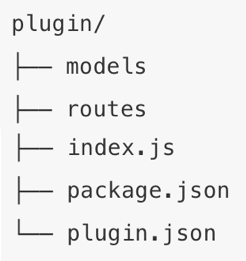
\includegraphics[width=0.35\textwidth]{./setup/arc}
\caption{Arquitectura de los plugins}
%\label{a:arquitectura}
\end{center}
\end{figure}

\subsubsection{Models}

En el caso de este proyecto no se creará ningún modelo de datos nuevo, ya que Aaaida dispone de un conjunto de modelos de datos que concuerda con el modelo que se necesita. El modelo elegido será Value, que cumple todas las necesidades de las medidas realizadas.

Los campos utilizados son los siguientes:

\begin{verbatim}
{
    value: {type: String},
    user: {type: mongoose.Schema.Types.Mixed, ref: 'User'},
    bond: {type: mongoose.Schema.Types.Mixed, ref: 'Bond'},
    measure: {type: mongoose.Schema.Types.Mixed, ref: 'Measure'},
    tags: {type: String},
    measured_at: {type: Date, readonly: true}
}
\end{verbatim}
\pagebreak

\begin{itemize}
\item value: Será el valor de la medida de ritmo cardiaco registrada. 
\item user: El usuario con el cual se está logueado en Aaaida
\item bond: Sería el “paciente” al cual se le toma la medida.
\item tags: Este campo se utiliza para diferenciar de qué aplicación pertenecen los valores.  
\item measured at: El instante que se tomó el valor. 
\end{itemize}

\subsubsection{Routes}

En el caso de que fuese necesario obtener información más concreta sobre el
modelo de datos, se deberían de definir cada una de esas rutas en la carpeta
routes del plugin. Como se dijo, route-injector genera automáticamente el CRUD para el modelo Values, pero necesita una ruta específica para ejecutar la conexión vía bluetooth con el sensor. 

Por lo tanto fue necesario la creación de la ruta, en el mismo fichero se copio todo el protocolo para la conexión con el sensor Zephyr. 

\begin{verbatim}
module.exports.route = function (router) {
   router.get('/coiote/media', function (req, res) {
       connect(function (media) {
           console.log("Tu HR media = " + media);
           res.json(media)
       });
   });
};
\end{verbatim}

Como se puede apreciar en el código una petición \texttt{get} a \texttt{ /coiote/media } ejecutará la función \texttt{connect} que establece la comunicación y recolección de datos.  

\subsubsection{Index}

En el siguiente fichero se configuran las funciones iniciales del plugin una vez
este ha cargado.

\begin{verbatim}
module.exports.config = require('./plugin.json');

module.exports.init = function (conf) { 
};
\end{verbatim}

El plugin no debe hacer ninguna función al iniciarse, por lo tanto, no debemos añadir nada en este fichero.
\pagebreak
\subsubsection{Package} 

En este fichero, se describe toda la información necesaria del paquete. 

\begin{verbatim}
{
 "name": "coiote-plugin",
 "version": "0.0.1",
 "description": "Plugin for CoIoTe",
 "dependencies": {
   "bluetooth-serial-port": "^2.0.0",
   "crc": "^3.4.0"
 }
}
\end{verbatim}

Se puede apreciar las 2 dependencias a módulos externos nombrados anteriormente. 

\subsubsection{Plugin} 

En este fichero, se indica el nombre del plugin y el directorio donde se encuentran
las rutas estáticas. Sirve para especificar dónde se encuentran todas esas rutas generadas para el plugin y no han sido creadas automáticamente por route-injector. 

\begin{verbatim}
{
 "name": "CoIoTe",
 "routes": ["routes"]
}
\end{verbatim}

\subsection{Creación de la página}

Una vez el plugin está creado, se necesitará crear la página web donde poder visualizar en la consola de Aaaida los resultados obtenidos de las medidas. 

Para esto se seguirá un proceso similar al de crear un plugin, pero en el directorio de \texttt{pages}, que tiene una arquitectura base similar a la siguiente:  

\begin{figure}[htb]
\begin{center}
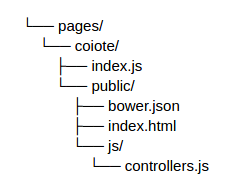
\includegraphics[width=0.35\textwidth]{./setup/arc2}
\caption{Arquitectura del directorio pages}
%\label{a:arquitectura}
\end{center}
\end{figure}


En este directorio, se encuentran definidos cada uno de los templates externos que se añadirán a la backoffice.

En este caso, ha sido necesario añadir el de coiote. En este directorio podemos encotrar el template index.js donde se define el controlador y como se visualiza en la consola de Aaaida y su URL. 

\begin{verbatim}
module.exports = {
   backoffice: true,
   url: 'coiote/mesures',
   template: 'coiote/index.html',
   controller: 'ChartCoioteController',
   menu: {
       clickTo: 'coiote/mesures',
       title: "mesures",
       section: "CoIoTe"
   }
   //backoffice: false // standalone website
};
\end{verbatim}

Creandonos una pestaña en la consola de Aaaida para el proyecto como podemos ver en la figura \ref{sec:coioteSec}. 

\begin{figure}[htb]
\begin{center}
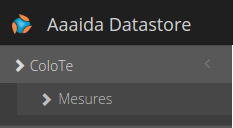
\includegraphics[width=0.25\textwidth]{./setup/arquitecturaCoiote}
\caption{Sección en la consola de Aaaida}
\label{sec:coioteSec}
\end{center}
\end{figure}

Una vez creado este fichero pasaremos a crear la template \texttt{index.html} y su controlador \texttt{controller.js}. En el controlador se realizan petición a las rutas creadas por route-injector para el modelo \texttt{value} y la ruta creada en el directorios \texttt{routes} para establecer la comunicación, y así poder rellenar el contenido de la plantilla.

La página para la visualización de los resultados sería esta:

\begin{figure}[htb]
\begin{center}
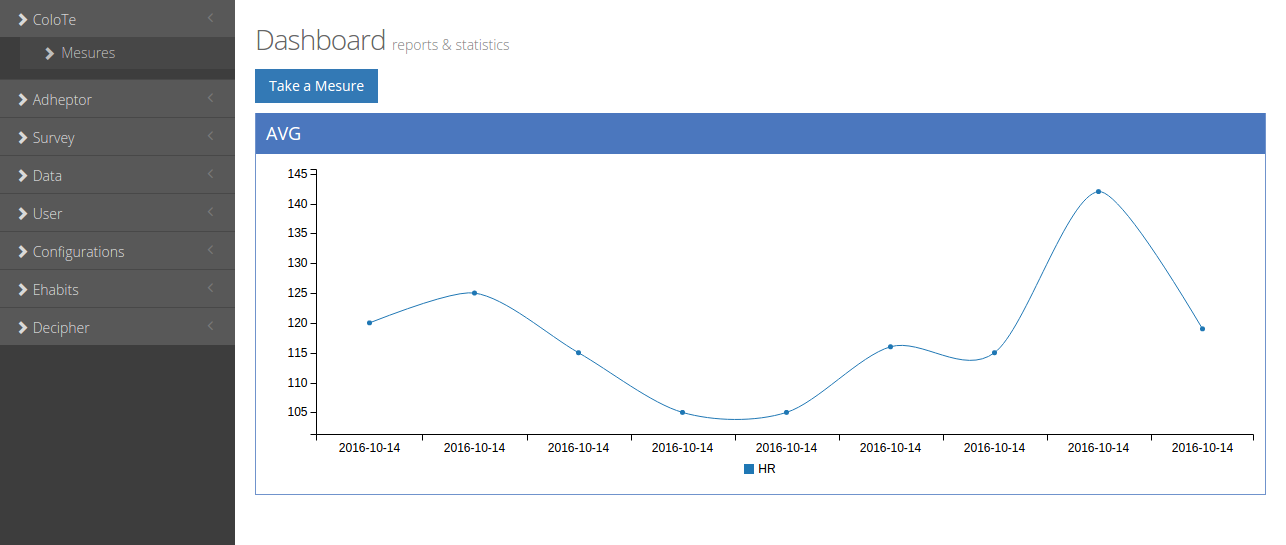
\includegraphics[width=1\textwidth]{./setup/visualizacionPaginaCoiote}
\caption{visualización de los datos en Aaaida}
%\label{sec:coioteSec}
\end{center}
\end{figure}
\pagebreak

\subsection{Recursos utilizados}

A continuación se mostrará en una tabla todos aquellos recursos de la API de Aaaida que fueron utilizados. 


\begin{table}[htb]

\begin{center}

\begin{tabular}{|c|c|c|}

\hline

{\bf Modelo} & {\bf Tipo} &

{\bf Ruta} \\ \hline \hline

Bond & get & /bond/:user.login  \\ \hline

Value & post & /values \\ \hline

Value & post & /value \\ \hline

- & get & /coiote/media \\ \hline

\end{tabular}

\caption{Exemple de taula}

\label{T:prova}

\end{center}

\end{table}

\begin{itemize}
\item Devuelve toda la información del usuario que está logueado en Aaaida.
\item Retorna los valores del bond del cual hemos tomado la medida.
\item Guarda el valor de la medida realizada. 
\item Establece la conexión y la recogida de datos.
\end{itemize}

\section{Despliegue en las Raspberry Pi}


\section{Conclusiones y Resultados}

Conseguir establecer la comunicación con el sensor fue una tarea para nada sencilla. Incluso haciendo tan solo la recogida de datos de una funcionalidad, se tuvo que entender muy bien cómo funcionaba y enviaba el sensor los datos. Sin contar que la documentación presentada por el fabricante se basaba únicamente en aplicaciones android. 

Como resultados, se desarrolló un protocolo de comunicación con el sensor, el cual nos proporcionaba la media  del ritmo cardiaco. La comunicación se podía ejecutar mediante la consola de Aaaida donde se visualizará el resultado y una vez validado se guardará en la base de datos. Para finalizar se proporciona una gráfica donde se puede ver un seguimiento de las medidas realizadas. 

\begin{figure}[htb]
\begin{center}
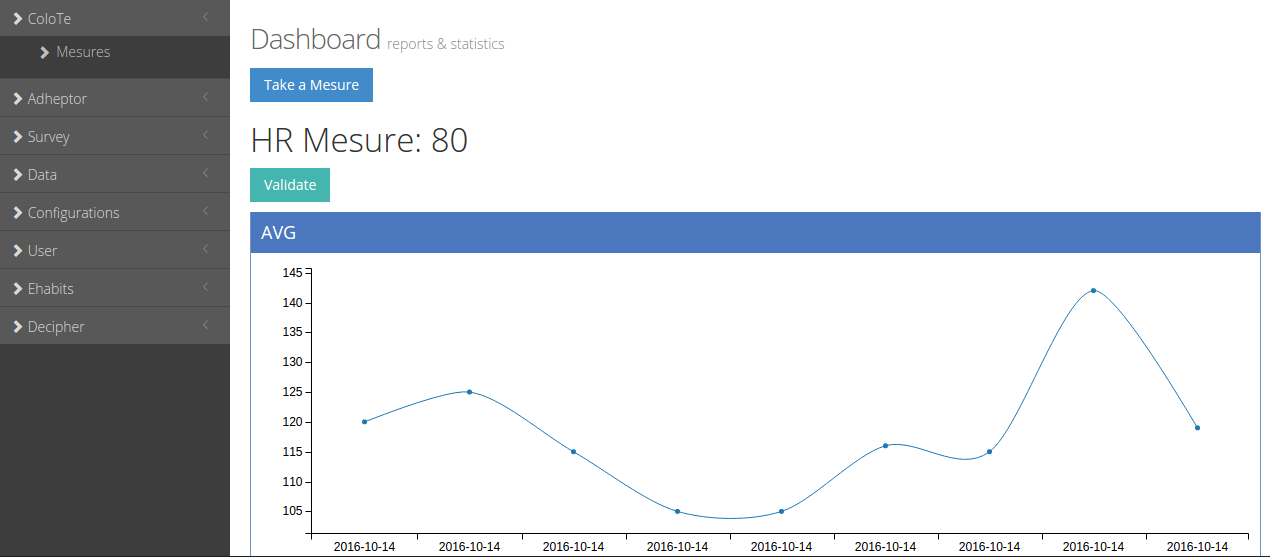
\includegraphics[width=1\textwidth]{./setup/final}
\caption{Consola de Aaaida}
%\label{sec:coioteSec}
\end{center}
\end{figure}
\pagebreak



\cleardoublepage
\phantomsection
\chapter*{Conclusiones}

Escriure aquí les conclusions del projecte. 

\chapter*{Glosario}

{\bf Journalig}: Memoria caché en la cual se tiene constancia de las escrituras hechas en disco. Esto en caso de fallo o desconexión no prevista ayuda a evitar la corrupción de datos. Por esta razón se activa, ya que la Raspberry Pi es un dispositivo sin batería y si hay un corte de luz, puede que se corrompa la base de datos y el restar no se pueda ejecutar. 

{\bf Daemon}: Proceso en segundo plano que se inicia como servicio.

{\bf API}: Application Programming Interface. Es un conjunto de especificaciones
para la comunicación entre diferentes componentes software.

{\bf IoT}: Internet Of Things

{\bf JSON}: Javascript Object Notation

{\bf MVC}: El modelo vista controlador, es un patrón de arquitectura de software que separa los
datos y la lógica de una interfaz de usuario y el módulo encargado de gestionar cada uno de sus
eventos y comunicaciones.

{\bf SPA}: Single-page Application, es una aplicación web que cabe en una sola página con el
objetivo de proporcionar una experiencia fluida a los usuarios.




%%%  BIBLIOGRAFIA
%%%%%%%%%%%%%%%%%%%%%%%%%%%%%%%%%%%%%%%%%%%%%%%%%%%%%%%%%%%%%%%%%%%%%%%%%%

%%% Per la bibliografia hi ha 2 opcions: generarla amb la utilitat BibTeX 
%%%                                      o fer-la ''a ma''
%%% NOTA: podeu trobar facilment informació sobre BibTeX a:
%%%  http://www.ctan.org/tex-archive/biblio/bibtex/contrib/doc/

%%% OPCIO 1: BibTeX (recomanat) -> descomentar les comandes seguents:
%\bibliographystyle{unsrt}   %% Estil de bibliografia EETAC
%\cleardoublepage
%\phantomsection
% Indicar aqui el(s) fitxer(s) que contenen la bibliografia
%\bibliography{fitxer1,...,fitxerN}  
%\pdfbookmark{Bibliografia}{sec:biblio}

%%% OPCIO 2: bibliografia manual
%%%
%%% L'argument d'entrada es el numero de referencies que s'inclouen
\cleardoublepage
\phantomsection
\begin{thebibliography}{2}

%% Llibres:  Autor/s (cognoms i inicials dels noms), títol del llibre (en cursiva), editor, ciutat i any de publicació. Quan es cita el capítol d'un llibre s'ha d'indicar el títol del capítol (entre cometes), el títol del llibre (en cursiva) i els números de pàgines amb la primera i la darrera incloses.

%%  Exemple de capitol en llibre
\bibitem{prova1} 
Turnbull, J. {\it The Docker book}.
(último acceso: 20 de 06 de 2016)

\bibitem{prova3} 
Humble, J. {\it Continuous Delivery}.
(último acceso: 20 de 06 de 2016)

\bibitem{prova4} 
Newman, S. {\it Building Microservices}.
(último acceso: 20 de 06 de 2016)

\bibitem{prova4} 
{\bf Web de Raspberry Pi}. URL: {\it https://www.raspberrypi.org/}
(último acceso: 17 de 10 de 2016)

\bibitem{prova4} 
{\bf Web de Docker}. URL: {\it https://www.docker.com}
(último acceso: 17 de 10 de 2016)

\bibitem{prova4} 
{\bf Blog de Hypriot}.  URL: {\it http://blog.hypriot.com/}
(último acceso: 17 de 10 de 2016)

\bibitem{prova4} 
{\bf Web de Alteraid}.  URL: {\it http://www.alteraid.com/}
(último acceso: 17 de 10 de 2016)

\bibitem{prova4} 
{\bf Web de MongoDB}.  URL: {\it https://www.mongodb.com/}
(último acceso: 17 de 10 de 2016)

\bibitem{prova4} 
{\bf Repositorio de Angular-chart}.  URL: {\it http://jtblin.github.io/angular-chart.js/}
(último acceso: 17 de 10 de 2016)

\bibitem{prova4} 
{\bf Repositorio de CRC}.  URL: {\it https://www.npmjs.com/package/crc}
(último acceso: 17 de 10 de 2016)

\bibitem{prova4} 
{\bf Repositorio de bluetooth-serial-port }.  URL: {\it https://www.npmjs.com/package/bluetooth-serial-port}
(último acceso: 17 de 10 de 2016)

\bibitem{prova4} 
{\bf Web de Zephyr, development tools }.  URL: {\it https://www.zephyranywhere.com/zephyr-labs/development-tools}
(último acceso: 17 de 10 de 2016)

\bibitem{prova4} 
{\bf Web de Qemu }.  URL: {\it http://wiki.qemu.org/Main Page}
(último acceso: 17 de 10 de 2016)

\bibitem{prova4} 
{\bf Web de Vmware }.  URL: {\it http://www.vmware.com}
(último acceso: 17 de 10 de 2016)

\bibitem{prova4} 
{\bf GitHub }.  URL: {\it https://github.com}
(último acceso: 17 de 10 de 2016)

%%  Exemple de d'article en revista


\end{thebibliography}

%%%%%%%%%%%%%%%%%%%%%%%%%%%%%%%%%%%%%%%%%%%%%%%%%%%%%%%%%%%%%%%%%%%%%%%%%%
%%%%%%                           APENDIXS                         %%%%%%%%
%%%%%%%%%%%%%%%%%%%%%%%%%%%%%%%%%%%%%%%%%%%%%%%%%%%%%%%%%%%%%%%%%%%%%%%%%%
\pagestyle{empty}  % no tocar

%% Descomentar una de les dues línies següents, en funció de:
%%  a) els apendixs s'encuadernaran apart (amb portada) 
%%  b) els apendixs s'enquadernen amb el mateix projecte (sense portada). 
%% Recordeu que si tot el document (amb apèndixs) excedeix les 100 pagines 
%% s'ha d'enquadernar a part
%\appendix\ambportada
\appendix\senseportada


%%%%%%%%%%%%%%%%%%%%%%%%%%%%%%%%%%%%%%%%%%%%%%%%%%%%%%%%%%%%%%%%%%%%%%%%%%
%%%%%% INCLOURE A Psudo apt-get install texmakerARTIR D'AQUI TOTS ELS CAPÍTOLS DELS APENDIXS   %%%%%%%%
%%%%%%%%%%%%%%%%%%%%%%%%%%%%%%%%%%%%%%%%%%%%%%%%%%%%%%%%%%%%%%%%%%%%%%%%%%

\chapter{Exemple de prova d'un apèndix}

Text de prova

\chapter{Ficheros utilizados}

Todos los ficheros utilizados y modificados para realizar el despliegue. 

\section{Fichero entrypoint}
\begin{verbatim}
function wait {
    echo -n "waiting for TCP connection to $1:$2..."
    while ! nc -w 1 $1 $2 2>/dev/null
    do
        echo -n .
        sleep 1
    done
    echo 'ok'
}
function startup {
    list=$(env | grep DOCKER_ | grep _TCP= | cut -d = -f 2)
    elems=($list)
    for key in "${!elems[@]}"
    do
        str=${elems[$key]}
        str2=${str#"tcp://"}
        IFS=:
            array=($str2)
        unset IFS
        host=${array[0]}
        port=${array[1]}
        wait $host $port
    done
}
startup
node bin/www
\end{verbatim}

\section{Script build rpi image}
\begin{verbatim}
#!/bin/bash
getVersion(){
    echo $(node -p -e "require('./package.json').version");
}
echo "Building image for version $(getVersion)"
echo "Installing dependencies"
npm install
echo "Downloading bower components for stats page"
cd stats
bower install --allow-root
cd ..
VERSION=getVersion
docker build -t alteraid/aaaida-datastore-arm -f scripts/rpi_docker/Dockerfile .
\end{verbatim}

\section{Dockerfile modificado}
\begin{verbatim}
FROM ioft/armhf-debian
RUN apt-get update; apt-get -y install curl; 
apt-get install libbluetooth3; apt-get -y install bluez

RUN set -ex \
  && for key in \
    9554F04D7259F04124DE6B476D5A82AC7E37093B \
    94AE36675C464D64BAFA68DD7434390BDBE9B9C5 \
    0034A06D9D9B0064CE8ADF6BF1747F4AD2306D93 \
    FD3A5288F042B6850C66B31F09FE44734EB7990E \
    71DCFD284A79C3B38668286BC97EC7A07EDE3FC1 \
    DD8F2338BAE7501E3DD5AC78C273792F7D83545D \
    B9AE9905FFD7803F25714661B63B535A4C206CA9 \
    C4F0DFFF4E8C1A8236409D08E73BC641CC11F4C8 \
  ; do \
    gpg --keyserver ha.pool.sks-keyservers.net --recv-keys "$key"; \
  done

ENV NODE_VERSION 4.4.5

RUN curl -SLO "https://nodejs.org/dist/v$NODE_VERSION/node-v$NODE_VERSION-
linux-armv7l.tar.gz" \
  && curl -SLO "https://nodejs.org/dist/v$NODE_VERSION/SHASUMS256.txt.asc" \
  && gpg --batch --decrypt --output SHASUMS256.txt SHASUMS256.txt.asc \
  && grep " node-v$NODE_VERSION-linux-armv7l.tar.gz\$" SHASUMS256.txt | 
  sha256sum -c - \
  && tar -xzf "node-v$NODE_VERSION-linux-armv7l.tar.gz" -C /usr/local 
  --strip-components=1 \
  && rm "node-v$NODE_VERSION-linux-armv7l.tar.gz" SHASUMS256.txt.asc 
  SHASUMS256.txt

COPY scripts/rpi_docker/entrypoint /entrypoint
RUN mkdir /aaaida
WORKDIR /aaaida
CMD ["/entrypoint"]

EXPOSE 40000

COPY . /aaaida
\end{verbatim}

\section{Docker-compose.yml modificado}
\begin{verbatim}
version: '2'
services:
 mongo:
  container_name: mongo
  restart: always
  image: partlab/ubuntu-arm-mongodb
  ports:
   - "27017:27017"
  volumes:
   - mongo-data:/data/db
  command: /usr/bin/mongod --smallfiles --journal
 aaaida:
  container_name: aaaidaArm
  restart: always
  network_mode: "home"
  privileged: true
  image: alteraid/aaaida-datastore-arm
  ports:
   - "40000:40000"
  environment:
   - NODE_ENV=docker
  volumes:
   - aaaida-data:/mnt/aaaidajs/

volumes:
 mongo-data:
   driver: local
 aaaida-data:
   driver: local  
\end{verbatim}


%%%%%%%%%%%%%%%%%%%%%%%%%%%%%%%%%%%%%%%%%%%%%%%%%%%%%%%%%%%%%%%%%%%%%%%%%%
%%%%%%%%%%%%%%%%%%%%%%%%%%%%%%%%%%%%%%%%%%%%%%%%%%%%%%%%%%%%%%%%%%%%%%%%%%
%%%%%%%%%%%%%%%%%%%%%%%%%%%%%%%%%%%%%%%%%%%%%%%%%%%%%%%%%%%%%%%%%%%%%%%%%%
% i  aixo es tot! ;)
\end{document}






